\chapter{Local Alignment of Squiggles}

\label{kap:align}

\theoremstyle{definition}
\newtheorem{definition}{Definition}[section]

% macro definitions
\newcommand{\ungap}{\textsc{ungap}}
\newcommand{\subseq}{|}
% end of macro definitions


Alignment algorithms play a role of great significance in the computational biology domain as it is one of the most basic ways of assessing similarity of sequences of DNA, RNA or proteins \cite{Durbin1998}.

In this chapter we will be dealing with algorithms that operate with pairs of sequences, hence the term \textit{pairwise}\footnote{There is also a variety of extensions of presented algorithms that perform multiple sequence alignments.}. We distinguish two fundamental types of alignment, namely \textit{global} and \textit{local}, differing in the restriction on the allowed scope of the output.

To avoid any misinterpretations, we will give a formal definition of the two types of alignments. The terminology that we use to talk about biological sequences is similar to that of formal languages. Firstly, we will define the necessary preliminaries.

\begin{definition}[Alphabet] An \textit{alphabet} $\Sigma$ is a nonempty set of elements we call \textit{symbols}.
\end{definition}

\begin{definition}[Sequence] A \textit{sequence} $S = s_1...s_n$ is a word over an alphabet $\Sigma$. We refer to $|S| = n$ as the \textit{length} of the subsequence.
\end{definition}

\begin{definition}[Subsequence] A \textit{subsequence} $S' = s_{i_1}s_{i_2}...s_{i_k}$ of a sequence $S = s_1...s_n$ is a sequence where $1 \leq i_j < i_{j+1} \leq n$ for each $1 \leq j \leq k-1$.
\end{definition}

\begin{definition}[Substring, Prefix, Suffix] We call a sequence $S' = s_{i},s_{i+1}...s_{i+k-1}$ a \textit{substring} of a sequence $S = s_1,...,s_n$, where $1 \leq k \leq n$ and $1 \leq i \leq n-k$. We also distinguish two special cases of substrings: the \textit{prefix} for which $i = 1$ and \textit{suffix} for $j = n$. We denote the substring relation as $\prec$.
\end{definition}

\begin{definition}[Iteration] Let $\Sigma$ be an alphabet. We denote $\Sigma^*$ to be the set of all finite sequences over $\Sigma$.
\end{definition}

To describe an alignment of two sequences, we will require a symbol called \textit{gap}. The gap is not an element of the alphabet and we will denote it with a $-$.

%\begin{definition}[Ungap] Let $\Sigma$ be an alphabet. The function $\ungap ~:~ (\Sigma \cup -)^* \to \Sigma$ that maps the gap symbols to $\varepsilon$ and is identity on all other symbols is called an \textit{ungap} function.
%\end{definition}


\section{Alignment of Nucleotide Sequences}
\subsection{Global Alignment}
\begin{definition}[Global pairwise alignment]
Let $X_1 = x_{1,1},...,x_{1,n}$, $X_2 = x_{2,1}, ..., y_{2,m}$ be sequences over an alphabet $\Sigma$ and $\max(n,m) \leq \ell \leq m+n$. A matrix $A_{2 \times \ell}$ is a \textit{global alignment} of sequences $X_1, X_2$ if the following four conditions hold:

\begin{enumerate}[(i)]
    \item $a_{i,j} \in (\Sigma \cup \{-\})$
    \item $X_i$ is a subsequence of $a_{i,1},...,a_{i,\ell}$ for $i=1,2$
    \item $|\{j ~|~ a_{i,j} = `-`\}| = \ell - |X_i|$ for $i=1, 2$
    \item $a_{1, j} \in \Sigma$ or $a_{2, j} \in \Sigma$ for $j = 1,...,\ell$
\end{enumerate}
\end{definition}

The global alignment of sequences $X,Y$ is therefore an arrangement of $X,Y$ with the possibility of gap insertion.

\begin{definition}[Set of all global alignments] Let $X = x_1,...,x_n$, $Y = y_1, ..., y_m$ be sequences over the same alphabet. Then we denote $\mathcal{A}(X,Y)$ to be the set of all global alignments of $X$ and $Y$.
\end{definition}

At this point we have defined all the necessary fundamentals to introduce the main goal of the global alignment problem:

\begin{definition}[Score function, Optimal global pairwise alignment]
Let $X = x_1,...,x_n$, $Y = y_1, ..., y_m$ be sequences over alphabet $\Sigma$ and let $s: (\Sigma \cup \{-\})^2 \to \mathbb{R}$ be a function called \textit{score} (or \textit{score function}). Then the optimal alignment $A_{\text{global}}^{\ast}$ with regards to score function $s$ is defined as

\begin{equation}
    A_{\text{global}}^{\ast} = \arg \max_{A \in \mathcal{A}(X,Y)} s(A_{1}, A_{2}) = \arg \max_{A \in \mathcal{A}(X,Y)} \sum_{i=1}^{\ell} s(a_{1i}, a_{2i})
\end{equation}
\end{definition}

In other words, we look for such an alignment of sequences $X, Y$ that maximizes the value of some score function $s$ (sometimes also called a \textit{scoring scheme}). For the choice of $s$, we intend to find biologically plausible alignments and therefore devise $s$ in such a way that encourages alignments on equals symbols and to the contrary, penalizes misalignments and alignments to gaps. The basic example of such scoring function is:

\begin{equation}
s(x, y) =
\begin{cases} 
    1, & \text{if } x = y\\
    -1, & \text{if } x \neq y\\
    -1, & \text{if } x = `-` \text{ or } y = `-`
\end{cases}
\label{basic_score}
\end{equation}

Let us now examine the cardinality of $\mathcal{A}(X,Y)$. From the definition of global alignment it should be obvious that the set is finite. For simplicity, let us assume that $|X| = |Y| = n$. Upon further examination we get \cite{Durbin1998}:

\begin{equation}
    |\mathcal{A}(X,Y)| = \binom{2n}{n} = \frac{(2n)!}{(n^2)!} \overset{(1)}{\simeq} \frac{2^{2n}}{\sqrt{\pi n}}
\end{equation}

where $(1)$ is the use Stirling's approximation\footnote{\url{https://en.wikipedia.org/wiki/Stirling\%27s_approximation}} of factorial. Clearly, the number of all global alignments grows rapidly and it is infeasible to search for the optimal solution by brute-force. Fortunately, a significantly more efficient approach exists.

\subsection*{Needleman–Wunsch Algorithm}
The algorithm developed by Saul B. Needleman and Christian D. Wunsch in $1970$ \cite{NeedlemanWunsch} provides an efficient way of finding a global alignment of two sequences (e.g. nucleotide or protein, but is applicable to any discrete domain). To do it efficiently, it makes use of the dynamic programming technique as one of the first algorithms in the bioinformatics domain.

Given two sequences $X = x_1,...,x_n, Y = y_1,...,y_m$, the structure of optimal subsolutions is defined by $\textbf{NW}[i, j]$ being the value of the optimal alignment of sequences $x_1...x_i$ and $y_1...y_j$. For each $i \in \{0, ..., n\}, j \in \{0, ..., m\}$,

\begin{equation}
\textbf{NW}[i, j] = \max
\begin{cases} 
    \textbf{NW}[i - 1, j - 1] + s(x_i, y_j), & \text{if } x_i \text{ is aligned to } y_j\\
    \textbf{NW}[i, j - 1] - 1, & \text{if } x_i \text{ is aligned to a gap}\\
    \textbf{NW}[i - 1, j] - 1, & \text{if } y_j \text{ is aligned to a gap}.
\end{cases}
\end{equation}


The trivial cases are $\textbf{NW}[i, 0] = -i$ and $\textbf{NW}[0, j] = -j$ for  $0 \leq i \leq n$ and $0 \leq j \leq m$. The value $\textbf{NW}[n, m]$ then holds the score of the optimal alignment. If the desired output is not only the score of the optimal alignment, but also the optimal alignment itself, its construction is carried out by a common approach among dynamic programming algorithms: we record the decisions of the algorithm throughout all its iterations and then process them backwards from the configuration at optimum. Formally, we construct another matrix $\textbf{B}_{n \times m}$, such that

\begin{equation}
\textbf{B}[i, j] = \arg \max
\begin{cases} 
    \textbf{NW}[i - 1, j - 1] + s(x_i, y_j), & \text{if } x_i \text{ is aligned to } y_j\\
    \textbf{NW}[i, j - 1] - 1, & \text{if } x_i \text{ if aligned to } `-`\\
    \textbf{NW}[i - 1, j] - 1, & \text{if } y_j \text{ if aligned to } `-`.
\end{cases}
\end{equation}

The matrix \textbf{B} allows us to compute an \textit{alignment path} which we now define.

\begin{definition}[Alignment path]
A sequence $(0, 0) = p_0,p_1, ..., p_{\ell} = (n, m)$ is an \textit{alignment path} if $p_{k} = (i, j)$ such that $\textbf{B}[i, j] = p_{k-1}$ for $k = 1, ..., \ell$.
\end{definition}

The actual optimal alignment path can be then computed by starting in position $(n, m)$ and at each step $(i, j)$ moving to the direction of at $\textbf{B}[i,j]$. The construction of the optimal alignment can therefore be done in $O(nm)$ time, and so it is not asymptotically slower than computing the score of the optimum. 

\subsection{Local Alignment}
\begin{definition}[Local pairwise alignment]
Let $X_1 = x_{1,1},...,x_{1,m_1}$, $X_2 = x_{2,1}, ..., y_{2,m_2}$ be sequences over an alphabet $\Sigma$ and $0 \leq \ell \leq m_1+m_2$. A matrix $A_{2 \times \ell}$ is a \textit{local alignment} of sequences $X_1, X_2$ if the following four conditions hold:

\begin{enumerate}[(i)]
    \item $a_{i,j} \in (\Sigma \cup \{-\})$;
    \item A subsequence  $a_{i,j_1},...,a_{i,j_k}$ of all non-gap symbols of $a_{i,1},...,a_{i,\ell}$ is a substring of $X_i$ for $i=1,2$
    \item $a_{1, j} \in \Sigma$ or $a_{2, j} \in \Sigma$ for $j = 1,...,\ell$
\end{enumerate}
\end{definition}

Thus, we can view the local alignment as a weaker form of global alignment in which we allow alignments between any substrings of the input sequences. Using that notion we now define the optimal local alignment.

\begin{definition}[Optimal local pairwise alignment]
Let $X_1 = x_{1,1},...,x_{1,m_1}$, $X_2 = x_{2,1}, ..., y_{2,m_2}$ be sequences over alphabet $\Sigma$ and let $s: (\Sigma \cup \{-\})^2 \to \mathbb{R}$ be a \textit{score function}. Then the optimal local alignment $A_{\text{local}}^{\ast}$ with regards to score function $s$ is defined as

\begin{equation}
    A_{\text{local}}^{\ast} = \arg \max_{
        \substack{Y_1 \prec X_1 \\ Y_2 \prec X_2 \\ A \in \mathcal{A}(Y_1,Y_2)}
    } s(A_{1}, A_{2}) = \arg \max_{
        \substack{Y_1 \prec X_1 \\ Y_2 \prec X_2 \\ A \in \mathcal{A}(Y_1,Y_2)}
    } \sum_{1 \leq i,j \leq \ell} s(a_{1,i}, a_{2,j})
\end{equation}
\end{definition}

The fact that the $\max$ operator iterates over all substrings of $X_1, X_2$ and all possible global alignments between them indicates that the naive exhaustive search for the optimum would consume at least as much time as in global alignment. Surprisingly, the local alignment can be computed in a way similar to global alignment, without an increase of the asymptotic time complexity. 

\subsection*{Smith–Waterman Algorithm}
A Smith–Waterman algorithm \cite{SmithWaterman} constructs local alignment for two sequences $X = x_1,...,x_n, Y = y_1,...,y_m$ by filling a matrix $\textbf{SW}_{n \times m}$ by using dynamic programming in a fashion similar to Needleman-Wunsch algorithm. The value $\textbf{SW}[i, j]$ stands for the value of the optimal \textit{local} alignment of subsequences $x_1,...,x_i$ and $y_1,...,y_j$ that contains both $x_i$ and $y_j$. The recurrence relation is as follows:

\begin{equation}
\textbf{SW}[i, j] = \max
\begin{cases}
    \textbf{SW}[i - 1, j - 1] + s(x_i, y_j), & \text{if } x_i \text{ is aligned to } y_j,\\
    \textbf{SW}[i, j - 1] - 1, & \text{if } x_i \text{ if aligned to } '-',\\
    \textbf{SW}[i - 1, j] - 1, & \text{if } y_j \text{ if aligned to } '-',\\
    0, & \text{otherwise}.
\end{cases}
\end{equation}

We set $\textbf{SW}[i, 0] = \textbf{SW}[0, j] = 0$. As a base case, the optimal local alignment of an empty sequence to any nonempty sequence is $0$, because the optimal solution is the alignment of two empty sequences (aligning anything more would result in a negative score). The final score of the optimal local alignment is the maximum among the optimal local alignments ending at particular sequence positions, i.e.

\begin{equation}
\textbf{SW} = \max_{\substack{i ~\in~ \{0, ..., n\} \\ j ~\in~ \{0, ..., m\}}} \textbf{SW}[i, j]
\end{equation}

To construct the optimal alignment itself we proceed as in the Needleman-Wunsch, with the exception that we start in a point $(i, j)$ at which \textbf{SW} is maximal.

\subsection{Likelihood-based Scoring Methods}
\label{sec:likelihood_scoring}
The standard scoring scheme presented earlier ($1$ for a match, $-1$ for a mismatch or a gap) may not be very useful in many different biological domains. For example, we may have a prior expectation that nucleotide $A$ mutates to $T$ with higher probability than to $C$. The desired property of the scoring function is to take into account the probabilities of these mutations. Would we have a good intuition or prior knowledge about the nature of these mutations, we could design a scoring function with respect to the particular probabilities \cite{Durbin1998}. Since this is often not the case, we can instead design a scoring scheme of a slightly different meaning:

\begin{equation}
s(X, Y) = \frac{P(X, Y ~|~ H)}{P(X, Y ~|~ R)}
\label{eq:likelihood_ratio}
\end{equation}


where $P(X, Y ~|~ H)$ is the conditional probability that $X$ and $Y$ are homologous (hence the $H$) sequences and $P(X, Y ~|~ R)$ is the probability that $X$ and $Y$ are completely random, unrelated sequences (hence the $R$). The ratios of the type $\frac{P(X, Y ~|~ H)}{P(X, Y ~|~ R)}$ are called \textit{relative likelihoods}. The score in Eq. \ref{eq:likelihood_ratio} expresses the level of likelihood that the two sequences are homologous  rather than unrelated \cite{Durbin1998}. The problem is now reduced to calculating the individual probabilities. For the sake of simplicity we will not consider gaps and assume $|X|=|Y|=n$. Let us first address $P(X, Y ~|~ R)$. Let the probability of occurrence of symbol $\alpha$ be $p_{\alpha}$. We assume that the symbols occur independently at each position in the sequences. Thus, we can easily see that

\begin{equation}
P(X, Y ~|~ R) = P(X)P(Y) = \Bigg( \prod_{i=1}^n p_{x_i} \Bigg) \Bigg( \prod_{i=1}^n p_{y_i} \Bigg)
\end{equation}

Let us now move to the calculation of $P(X, Y ~|~ H)$. Let $p_{\alpha \beta}$ be the joint probability of the symbols $\alpha$ and $\beta$ occurring aligned in homologous sequences. From the biological perspective, we can think of symbols $\alpha, \beta$ as a derivation from a common ancestor, which had either $\alpha$ or $\beta$ at the particular position \cite{Durbin1998}. The said probability is therefore

\begin{equation}
P(X, Y ~|~ H) = \prod_{i=1}^n p_{x_i y_i}
\end{equation}

and that finalizes our calculation. Putting all together, we have

\begin{equation}
    \frac{P(X, Y ~|~ H)}{P(X, Y ~|~ R)} = \frac{\prod_{i=1}^n p_{x_i y_i}}{\prod_{i=1}^n p_{x_i}p_{y_{i}}}
\end{equation}

What remains to work out is how to obtain an additive scoring scheme from this probability ratio. It turns out that it suffices to take the logarithm of the expression:

\begin{multline}
\log\Bigg( \frac{P(X, Y ~|~ H)}{P(X, Y ~|~ R)} \Bigg) =
\log \Bigg( \frac{
\prod_{i=1}^n p_{x_i y_i} }
{\prod_{i=1}^n p_{x_i} \prod_{i=1}^n p_{y_i}} \Bigg) =\\
= \log \Bigg(\prod_{i=1}^n \frac{p_{x_i y_i}}{p_{x_i}p_{y_i}} \Bigg) =
\sum_{i=1}^n \log \Bigg( \frac{p_{x_i y_i}}{p_{x_i}p_{y_i}} \Bigg)
\label{eq:log_likelihood}
\end{multline}

The monotonicity of logarithm function guarantees the preservation of global extremes, which means that maximizing the logarithm of the original likelihood ratio does not change the result. Therefore, the score function for a pair of basis $x,y$ is defined as

\begin{equation}
s(x, y) = \log \Bigg( \frac{p_{x y}}{p_{x}p_{y}} \Bigg)
\end{equation}

which according to Eq. \ref{eq:log_likelihood} sums to the likelihood ratio as was desired. The ratio $\frac{P(X, Y ~|~ H)}{P(X, Y ~|~ R)}$ is called a \textit{log-odds} ratio and it is the standard approach for constructing scoring schemes, for example BLOSUM$50$ for protein sequences \cite{Durbin1998}. We call this type of a scoring scheme a \textit{log likelihood ratio scoring scheme}.

If we were to employ this concept in practice, we would require a sufficiently large database of aligned sequences from which we would be able to infer the discussed probabilities. 

The log likelihood ratio scoring scheme, however, differs from the notion we sketched at the beginning of this Chapter: the transition probabilities we spoke of are comprised in $P(X, Y ~|~ H)$ \cite{Durbin1998}.

\section{Global Alignment of Squiggles}
Up until this point we talked about discrete sequences, i.e. sequences over a finite alphabet. In this section we turn our focus to squiggles which are a special case of sequences because they are a discretization of continuous events. In squiggle alignments we do not use gaps, but map the values to values.

\subsection{Dynamic Time Warping}
Originally designed for speech recognition purposes, \textbf{D}ynamic \textbf{T}ime \textbf{W}arping (DTW) is a global alignment algorithm for finding alignments of time series \cite{kruskal1983overview}.

DTW is very similar to Needleman–Wunsch Algorithm, albeit the goal of DTW is to minimize a so called \textit{cost} rather than maximize \textit{score}. The cost is function $c(\cdot, \cdot)$ that assigns a real number to each pair of signal values. Typical example of a cost function used in DTW is the absolute value of difference. Consider two sequences $X = x_1,...,x_n, Y = y_1,...,y_m$, let $\textbf{DTW}[i, j]$ be the minimum cost of aligning sequences $X$ and $Y$. Then, similarly as in Needleman–Wunsch:

\begin{equation}
\textbf{DTW}[i, j] = c(x_i, y_j) + \min
        \begin{cases}
            \textbf{DTW}[i - 1, j - 1],\\
            \textbf{DTW}[i - 1, j],\\
            \textbf{DTW}[i, j - 1].\\
        \end{cases}
    \label{eq:dtw_recurrence}
\end{equation}

The base case is an alignment to an empty sequence, which we define to have a cost of $0$, so $\textbf{DTW}[i, 0] = \textbf{DTW}[0, j] = 0$ for $0 \leq i \leq n, 0 \leq j \leq m$. The construction of the optimal alignment follows the same steps as in Needleman-Wunsch.

\section{Local Alignment of Squiggles}
In the problem we aim to solve, we need to be able to compare squiggles by their barcode class as we stated in Chapter \ref{kap:outline}, i.e. some notion of a similarity on squiggles. As the barcodes are located near the starts (and ends) of squiggles (see Fig. \ref{fig:barcode_pos}), only sufficiently long prefixes (and suffixes) are of interest.

A standard approach to demultiplexing base called reads is to use a local alignment for the read ends, which would, in the ideal case, either yield a barcode match or an alignment to a random substring of the read. We could then decide the presence of the particular barcode by comparing the score of this alignment to some kind of a threshold, similarly to Albacore or Porechop \cite{Porechop}. This scenario would naturally only work only if the reads are base called without many errors and do not contain a substring that could be evaluated as a spurious barcode match.

Since local alignment is the key to barcode demultiplexing, we need to develop a DTW-like algorithm that would work similarly in the signal space. We base our idea on the Smith-Waterman algorithm for local alignment by maximizing some score function. Similarly as in Smith-Waterman, we add an option of starting a new alignment at any point with a score of $0$. The structure of this \textit{\textbf{L}ocal \textbf{D}ynamic \textbf{T}ime \textbf{W}arping} (LDTW) algorithm is as follows:

\begin{equation}
    \textbf{LDTW}[i, j] = \max
        \begin{cases}
            \textbf{LDTW}[i, j - 1] ~+~ s(x_i, y_j),\\
            \textbf{LDTW}[i - 1, j] ~+~ s(x_i, y_j),\\
            \textbf{LDTW}[i - 1, j - 1] ~+~ s(x_i, y_j),\\
            0
        \end{cases}
    \label{eq:ldtw_recurrence}
\end{equation}

Furthermore, we drop the possibility of aligning the actual value $x_i$ to value $y_j$ and therefore force a step of unit length in either direction of the alignment. This will ensure that for any two subsequences of $X$ and $Y$, all the possible  (global) alignments are of the same length, which reduces the number of potential alignments found  and consequently also the variance of the final scores. The final recurrence looks as follows:

\begin{equation}
    \textbf{LDTW}[i, j] = \max
        \begin{cases}
            \textbf{LDTW}[i, j - 1] ~+~ s(x_i, y_j),\\
            \textbf{LDTW}[i - 1, j] ~+~ s(x_i, y_j),\\
            0
        \end{cases}
    \label{eq:ldtw_recurrence_corrected}
\end{equation}

We now need to address the scoring function $s(\cdot, \cdot)$. The basic version of DTW aligns two time series so that the Euclidean distance between them is minimalized. At this point we see that we that using this cost function a score function in our local alignment would result in undesirable alignments only, because it would be always more beneficial to extend the actual alignment and gain a non-negative score. We therefore need a scoring scheme that would yield more reasonable alignments.

In fact, a scoring function $s(\cdot, \cdot)$ for a local alignment must satisfy these two necessary conditions to work desirably \cite{rosenberg2009sequence}:

Let $X, Y$ be random variables representing two symbols of the same alphabet. Then $s$ must satisfy:
\begin{enumerate}
    \item $P\big[s(X, X) > 0 \big] > 0$
    \item $\mathbb{E}\big[ s(X, Y) \big] < 0$
\end{enumerate}

The first condition ensures that it is possible to find an alignment of non-zero length. The need for the second condition can be explained on a pair of random, unrelated sequences: if the case was that $\mathbb{E}\big[ s(X, Y) \big] > 0$ then the algorithm could, in expectation, at any point extend the alignment and increase the score. This would lead to a tendency of aligning the whole lengths of sequences \cite{rosenberg2009sequence}.

To design a scoring scheme that would sufficiently measure the similarity of the squiggles we employ the likelihood ratio scoring scheme defined in Section \ref{sec:likelihood_scoring}. However, its application in our setting is not straightforward. First, we do not have a sensible way of comparing the signal values as we do with, for example, nucleobases. We can overcome this obstacle by reducing the dimension of the scoring function domain - instead of having a scoring function dependent on the pair of signal values, it will depend on the absolute distance between the values. The second issue we need to address, is the estimation and inference of the probabilities of types $p_{xy}$ and $p_x$, which we describe in the next section.

\subsection{Estimating the Probabilities}
The inference of the probabilities of type $p_x$ from Section \ref{sec:likelihood_scoring} in the context of our one-dimensional scoring scheme is relatively simple - we only need to sample a sufficiently large number of absolute distances of points from random positions in unrelated squiggles. Such squiggles can therefore also selected uniformly at random from the training set.

The more complicated case is with the probabilities of type $p_{xy}$, where for sampling of such probability we would in the 'ideal' case need a database of squiggle pairs already aligned on their barcode sections by some notion of a local alignment, which is not available to us. We can, however, empirically approximate this probability by performing conventional DTW alignments of the barcode squiggles belonging to the same class and sampling the distances from such DTW-aligned barcodes. Therefore, the probability ratio $\frac{P(X, Y ~|~ H)}{P(X, Y ~|~ R)}$ can be approximated as:

\begin{multline}
s(X, Y) =   \log \Bigg( \frac{P(X, Y ~|~ H)}{P(X, Y ~|~ R)} \Bigg) =
\sum_{x \in X, y \in Y} s(x, y) =\\=
\sum_{x \in X, y \in Y} \log \Bigg( \frac{P \big(|x - y|~ \text{occurs in aligned positions of barcodes}  \big)}{P \big(|x - y|~ \text{occurs in random positions of squiggles} \big)} \Bigg) =\\= \log \Bigg( \frac{P(|x-y| ~|~ H)}{P(|x-y| ~|~ R)} \Bigg) \approx \\ \approx
\sum_{x \in X, y \in Y} \log \Bigg(
\frac{P \big(|x - y|~ \text{occurs in DTW-aligned barcode squiggles} \big)}{P \big(|x - y|~ \text{occurs in random positions of squiggles} \big)} \Bigg)
\end{multline}

Provided that we have a 'training' dataset that consists of a set of barcode squiggles and another set of squiggles corresponding to unrelated sequences, we can sample the needed frequencies of distances according to the algorithm below:

\begin{algorithm}[H]
\floatname{algorithm}{Algorithm}
\renewcommand{\thealgorithm}{}
\caption{Approximation of $\frac{P(|x-y| ~|~ H)}{P(|x-y| ~|~ R)}$ }
\begin{algorithmic}[1]
\STATE $Dist_{aligned} \gets \{\}$
\FOR{$i = 1$ to $N_{\text{iter}}$}
\STATE $B_1 = b_{11}...b_{1n}, B_2 = b_{21}...b_{2m} \xleftarrow{\$} Barcodes$ // sample barcode signals uniformly at random
\STATE $Path \gets \textsc{DTW}(B_1, B_2)$
\STATE $Dist_{aligned} \gets Dist_{aligned} \cup \{~ |b_{1i} - b_{2j}| ~|~ (i,j) \in Path \}$
\ENDFOR
\STATE $Dist_{random} \gets \{\}$
\WHILE{$|Dist_{random}| < |Dist_{aligned}|$}
\STATE $S_1 = s_{11}...s_{1n}, S_2 = s_{21}...s_{2m} \xleftarrow{\$} Squiggles$ // sample read signals uniformly at random
\STATE $Dist_{random} \gets Dist_{random} \cup \{~ |s_{1i} - s_{2j}| ~|~ i,j~ \text{randomly chosen} \}$
\ENDWHILE
\STATE $\hat{P}(|x-y| ~|~ H) = P(|x-y| \in Dist_{aligned})$
\STATE $\hat{P}(|x-y| ~|~ R)= P(|x-y| \in Dist_{random})$
\end{algorithmic}
\end{algorithm} 
\bigskip

Even though we would 'train' (or perhaps more accurately, \textit{estimate}) our model using a number of particular barcodes, we hypothesize that our method should remain invariant to the barcodes being used, provided that they are pairwise sufficiently dissimilar. The robustness of our model would be the consequence of the fact that the model was exposed to a sufficient variety of dissimilarities in DTW alignments.

It is, however, hard to find any theoretical guarantees about how would such approximation actually perform, so naturally we will test this approach experimentally.

\subsection{Experimental Evaluation}
Our training dataset consists of several hundreds of squiggles labeled by the first $4$ barcodes of the Native Barcoding Kit. The squiggles are aggregated in a \texttt{HDF5} file and grouped by their barcode class. Each squiggle is annotated with the position of the start and end of its barcode sequence, so the extraction of the corresponding barcode squiggle is trivial. The construction of the training dataset is described in more detail in Section \ref{sec:datasets_handling}.

The resulting dataset contains more potential samples of distances from a single pair of reads when sampling $\hat{P}(|x-y| ~|~ R)$ than in the case of sampling $\hat{P}(|x-y| ~|~ H)$. In the first case we can, in theory, sample any pair of positions of the reads, while in the second case we are limited to the signal regions corresponding to barcodes, and only the pairs of positions that are aligned. We therefore first compute a set of aligned distances on a selected 'training' subset of squiggles and subsequently sample the same amount of distances from random positions of unrelated squiggles, as is outlined in the algorithm earlier.

We sampled $\approx 6.2$ mil. distances for both DTW-aligned positions and random positions from $75$ squiggles drawn from the training dataset. Subsequently, we the scoring function by the process summarized in the following pseudocode:
\begin{algorithm}[H]
\floatname{algorithm}{Algorithm}
\renewcommand{\thealgorithm}{}
\caption{LDTW scoring scheme construction}
\label{alg:scoring_preparation}
\begin{algorithmic}[1]
\STATE For both $Dist_{aligned}$ and $Dist_{random}$  construct a normalized histogram of the observed frequencies with each bar having a width of $0.1$
\STATE Take the ratio of the two histograms bar by bar
\STATE Take the $\log$ of the histograms ratio to obtain the additive scoring scheme
\end{algorithmic}
\end{algorithm} 
\bigskip

The construction of the scoring scheme is visualized in Fig. \ref{fig:scoring_scheme}.

\begin{figure}[!ht]
    \centering
    \subfloat[Pairwise distances histogram]
    {{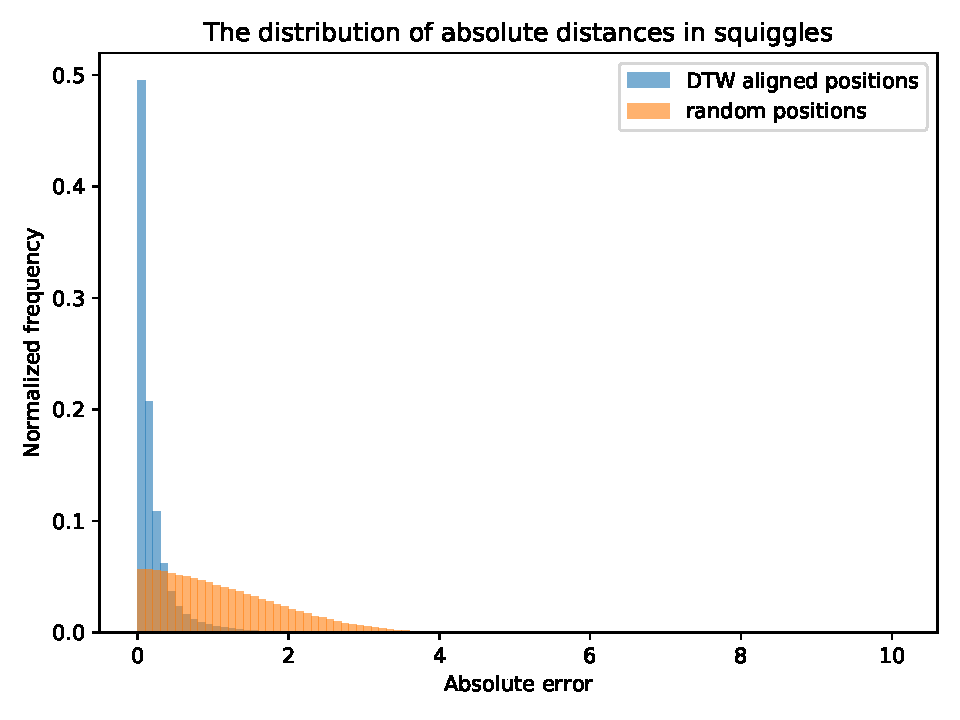
\includegraphics[width=7cm]{images/distance_histogram.pdf} }}%
    \qquad
    \subfloat[Scoring scheme]
    {{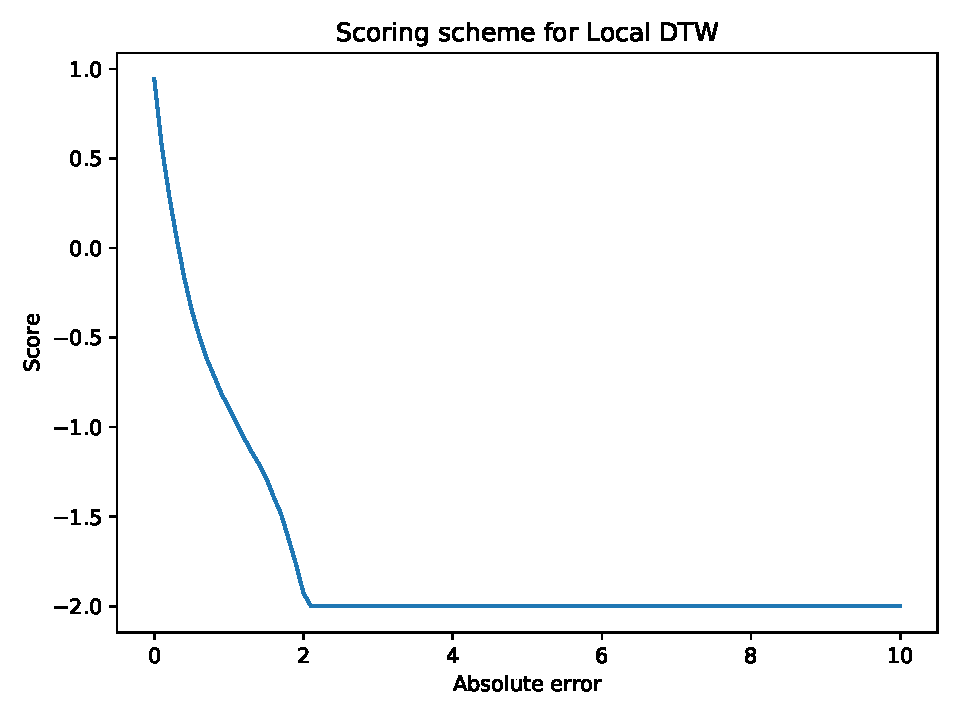
\includegraphics[width=7cm]{images/score_plot.pdf} }}%
    \caption[Scoring scheme construction.]{Left: Histogram of pairwise distances constructed from $\approx 6.2$ mil. aligned positions and the same amount of randomly chosen positions in the training squiggles. Right: Resulting scoring scheme plotted as a piecewise linear function with a segment length of $0.1$. The scores for distances bigger than $2.5$ are kept constant as the frequencies for these values were only non-zero due to the noise present in the signal.}%
    \label{fig:scoring_scheme}%
\end{figure}

With $\mathbb{E}\big[(s(\cdot, \cdot)\big] \approx -1.5$ and $s(x, y) > 0$ for $|x-y| \in [0, 0.4]$, our scoring scheme satisfies the necessary conditions we stated before.  However, when using this scoring scheme to align squiggles, we found that it performs rather poorly, resulting in a full length alignment for almost any pair of squiggles, yielding a very high final score regardless of a barcode match/mismatch. Most of the alignments were very similar to the one pictured in fig. \ref{fig:zero_delta_align}.

\begin{figure}[!ht]
    \centering
    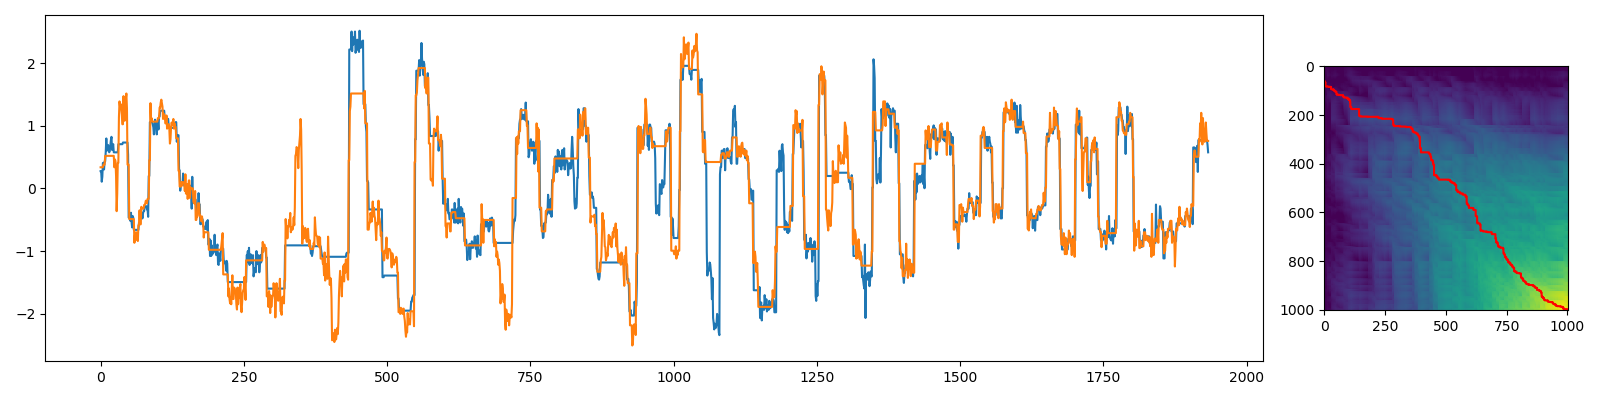
\includegraphics[width=15.5cm]{images/zero_delta_alignment.png}
    \caption[Basic LDTW alignment]{Left: LDTW alignment of squiggles from barcode classes $1$ and $2$. Right: Alignment matrix. We only expect short random alignments, yet the algorithm aligned the whole length of the window.}
    \label{fig:zero_delta_align}
\end{figure}

\subsection{Correction for Length}
As can be seen from the Fig. \ref{fig:delta_samples}  part $a)$, the barcode classes under such scoring scheme are not very well pronounced, the similarity scores often blending together where we should see clearly defined regions of classes. This could be explained by overestimation of our scoring scheme, which does not take into account the succession of signal values but only individual points.

Durbin et al. \cite{Durbin1998} proposes a method for solving a similar problem when using the log-likelihood ratio scoring scheme: in a setting where a pattern is searched for in a in a database by comparing a query sequence to database entries by local alignment, a logarithm of the length of the database entry is to be subtracted from the resulting alignment score. This corresponds to multiplying the resulting score by the apriori probability of the expected number of matching starting points. The correction reduces the growth of alignment scores to random sequences as their lengths increase. This is in accordance with the idea that in the ideal case, we would expect similarly low scores to random sequences regardless of the sequence length. Similarly to Durbin et al., we would expect the LDTW alignment scores of random, unrelated squiggles to be low regardless of their lengths.

We will establish an approach similar to Durbin et al. by introducing a new term $\delta$ that we will subtract from the absolute distance of the points before evaluating the original score function. The new score function $s'(\cdot, \cdot)$ will therefore look as follows:

\begin{equation}
    s'(x, y) = f(|x-y| - \delta)
\end{equation}

where $f$ is the score function in terms of the absolute distance as in Fig. \ref{fig:scoring_scheme} b).

Even though the parameter $\delta$ may be diffucult to compute, we can estimate its value using an exhaustive search on our training set for a discretization of $\delta$ in $\{0, 0.1, 0.2, ..., 1\}$. In particular, we extracted the squiggle prefixes of $1000$ values in length and computed the LDTW scores of all pairs of the training squiggles, both intra- and inter- barcodes.

From these histograms we would like to estimate the underlying density functions of the scores so that we can examine the measure of separation between those two score categories. This can be done by a non-parametric\footnote{non-parametric methods do not assume that the probability density distribution they work with is normal} method called Kernel density estimation (KDE). The concept was brought independently by Murray Rosenblatt \cite{davis2011remarks} and Emanuel Parzen \cite{parzen1962estimation} and its main idea is as follows:

Given a set of independent and identically distributed (i.i.d.) random variables $X_1, ..., X_n$ with a probability distribution function (PDF) $F(x)$ and a density function $f(x)$, we would like to estimate $f(x)$ from a set of observations of $X_1, ..., X_n$. E. Parzen \cite{parzen1962estimation} proposed to estimate the density as

\begin{equation}
\hat{f_n}(x) = \int_{-\infty}^{\infty} \frac{1}{h} K_h \Big(\frac{x-y}{h} \Big) dF_n(y) = \frac{1}{nh} \sum_{i=1}^n K_h \Bigg( \frac{x-X_i}{h} \Bigg)
\end{equation}

where $K_h$ is a so called \textit{kernel function}. Kernel functions (or just kernels) are a special class of functions that are constant on almost all of their domains, but exploit some non-trivial behavior on a segment of its domain. This segment is called a \textit{window}. Kernels are usually parametrized by their windows size $h$, the parameter is being called a \textit{bandwidth}. The size of the bandwidth controls the trade off between the bias and the variance of the estimation \cite{kerneldensity}. In our case we are using a \textit{Gaussian kernel} defined as

\begin{equation}
    K_h(x) = \exp \Big(- \frac{x^2}{2h^2} \Big).
\end{equation}

We set the bandwidth size to $10$ to filter out most of the noise in the data. The resulting score histograms together with their probability density estimations by KDE can be seen in Fig. \ref{fig:deltas_collage}. As an alternative way of visualization, we also plotted the score distributions in terms of $\delta$ in the form of an ensemble of double boxplots in Fig. \ref{fig:delta_boxplot}. We examined the measure of the overlap of score distributions between intra-barcode and inter-barcode pairs, using the Bhattacharyya coefficient $\textbf{BC}$ \cite{derpanis2008bhattacharyya} defined as

\begin{equation}
    \textbf{BC}(p, q) = \sum_{x} \sqrt{p(x)q(x)},
\end{equation}


where $p, q$ are the measured probability distributions. Bahattacharyya coefficient is a frequently used tool in computer vision, used mainly in comparing histograms of features, e.g. colors from a particular segment \cite{derpanis2008bhattacharyya}. It is easy to see that the range of \textbf{BC} is the interval $[0, 1]$. \textbf{BC} is closely related to the Hellinger distance, which itself has a natural geometric representation - it is the Euclidean distance of the two points projected by distribution vectors on the surface of a unit sphere \cite{harmanPersonal}.

We will also use a second metric: the area of the overlap relative to the combined area of the two distributions. The \textbf{o}verlap \textbf{a}rea \textbf{OA} is therefore:

\begin{equation}
    \textbf{OA}(p, q) = \int_{-\infty}^{\infty} \min(p(x), q(x)) ~dx \stackrel{(\star)}{=}  \sum_x \min(p(x), q(x))
\end{equation}

where $(\star)$ holds due to the densities $p(x), q(x)$ being discrete. Clearly $0 \leq \textbf{OA} \leq 1$, where $\textbf{OA} = 0$ means no overlap at all and $\textbf{OA} = 1$ means that the distributions are identical.

\begin{table}[!ht]
\centering
\begin{tabular}{|c|cccccccc|}
\hline
$\delta$ & 0 & 0.1  & 0.2  & 0.3  & 0.4  & 0.5  & 0.6  & 0.7\\
\hline
\textbf{BC} & 0.86  & 0.85 & 0.84 & 0.83 & 0.81 & 0.80 & 0.88 &  0.79\\  \hline
\textbf{OA}  & 0.56 & 0.55 & 0.54 & 0.53 & 0.50 & 0.47 & 0.64 & 0.77\\  \hline
\end{tabular}
\caption{\textbf{BC} and \textbf{OA} coefficients for different values of $\delta$.}
\label{tab:delta_measures}
\end{table}

\begin{figure}[!ht] % "[t!]" placement specifier just for this example
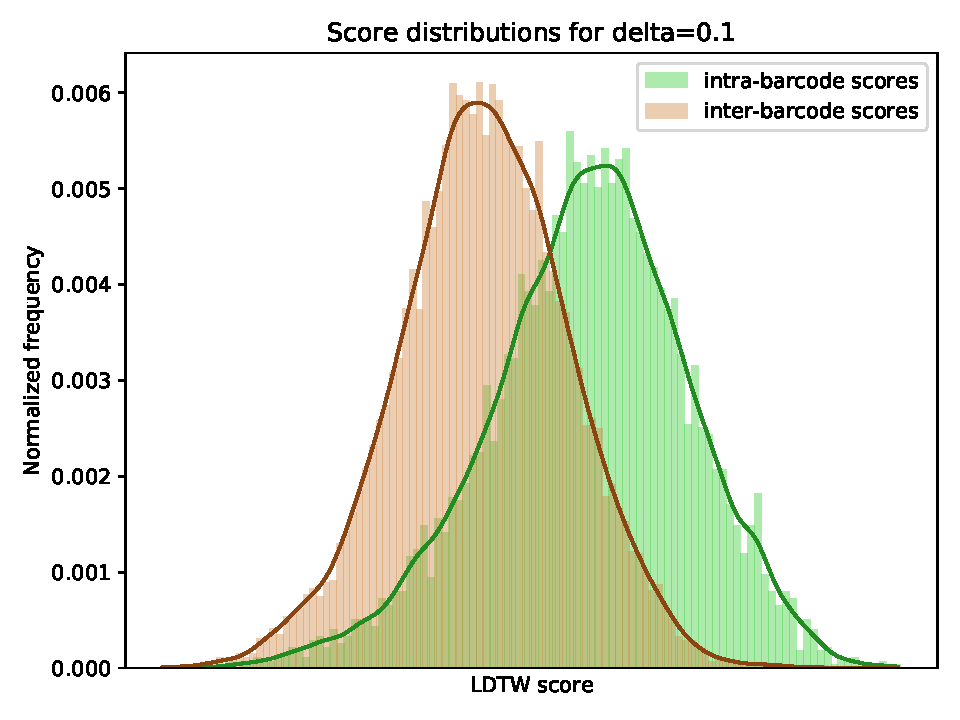
\includegraphics[scale=0.5]{images/delta/delta_raw_10.pdf}
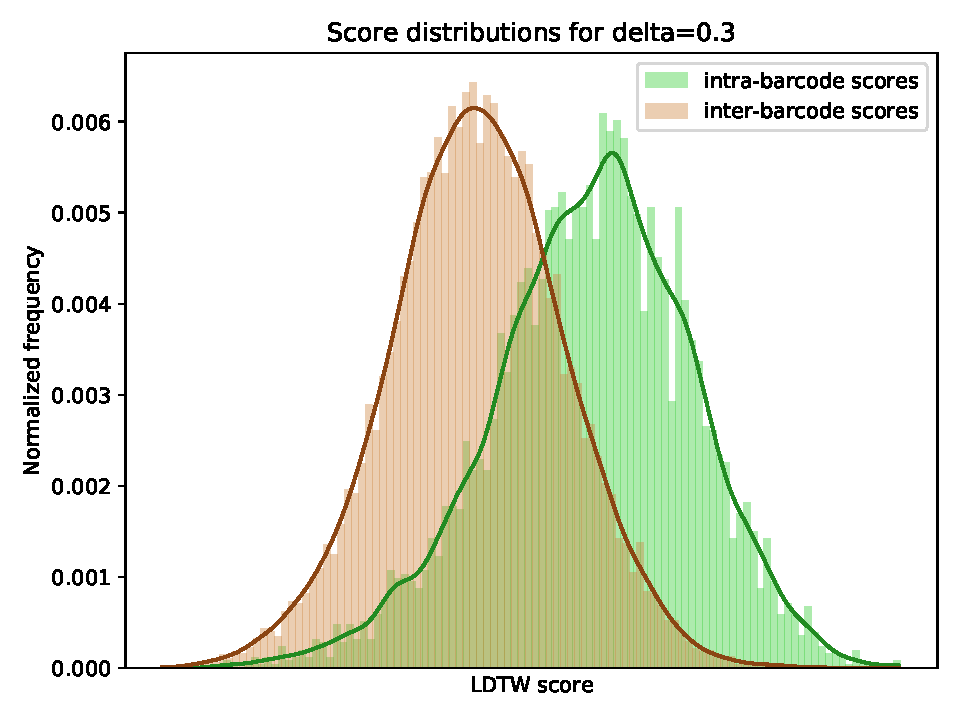
\includegraphics[scale=0.5]{images/delta/delta_raw_30.pdf}

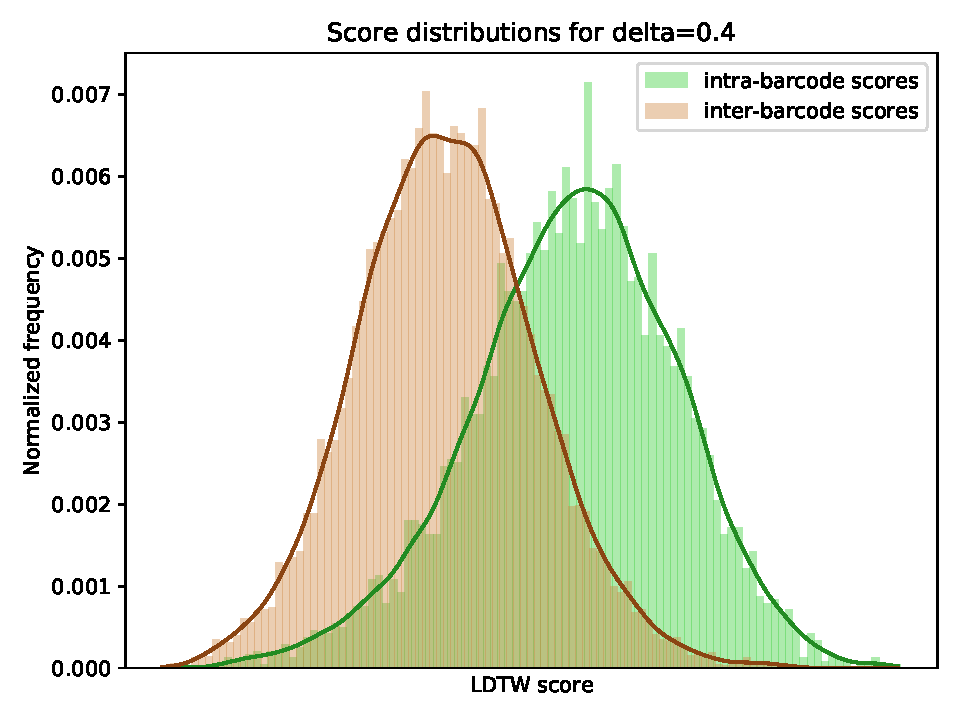
\includegraphics[scale=0.5]{images/delta/delta_raw_40.pdf}
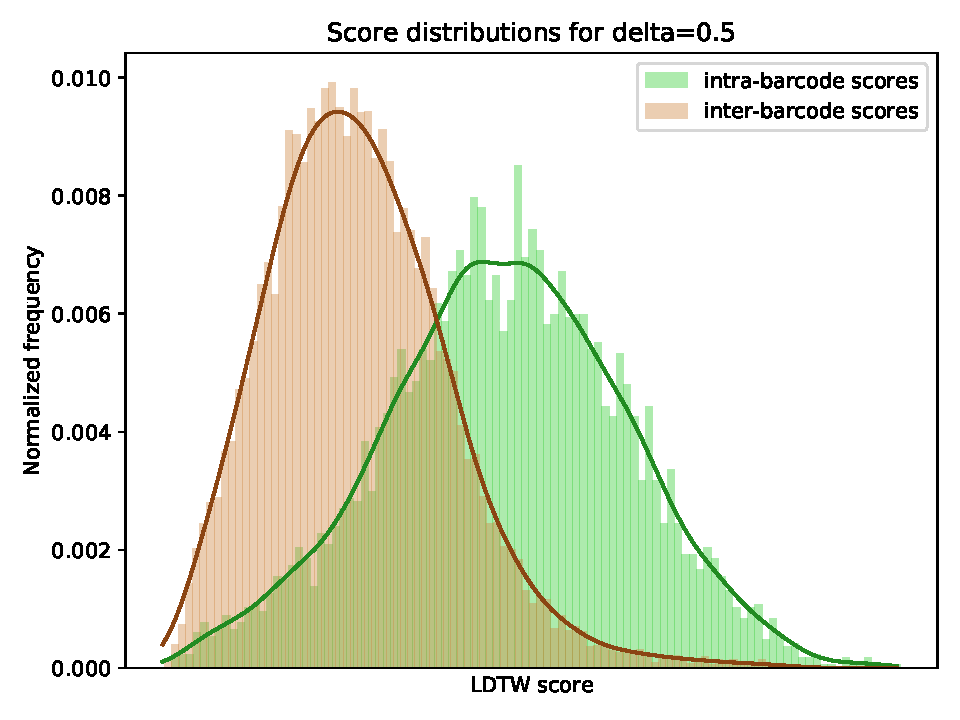
\includegraphics[scale=0.5]{images/delta/delta_raw_50.pdf}

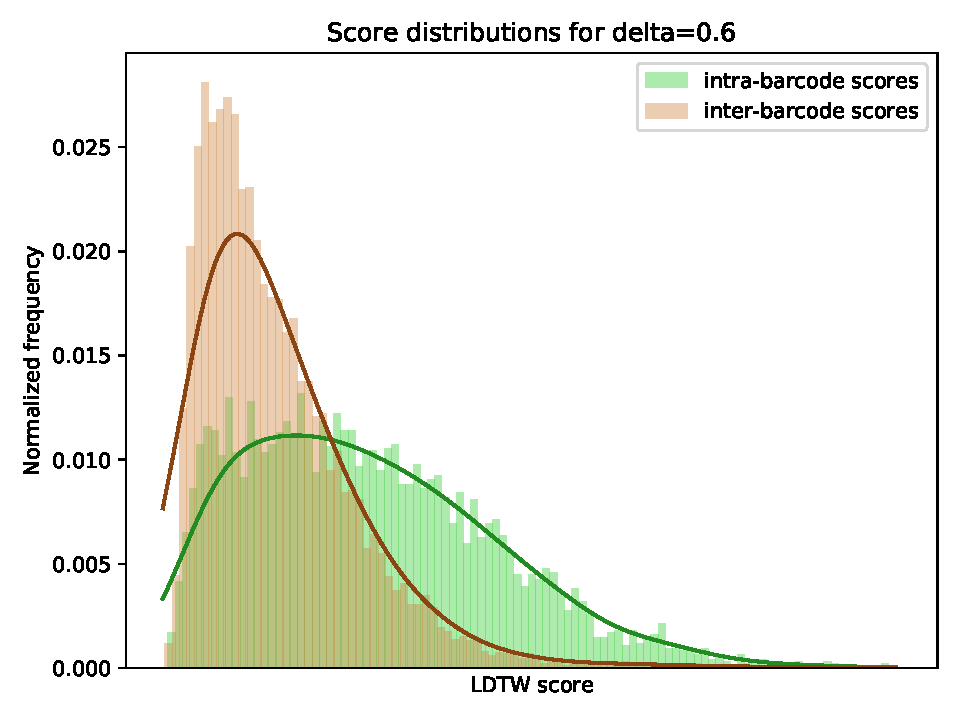
\includegraphics[scale=0.5]{images/delta/delta_raw_60.pdf}
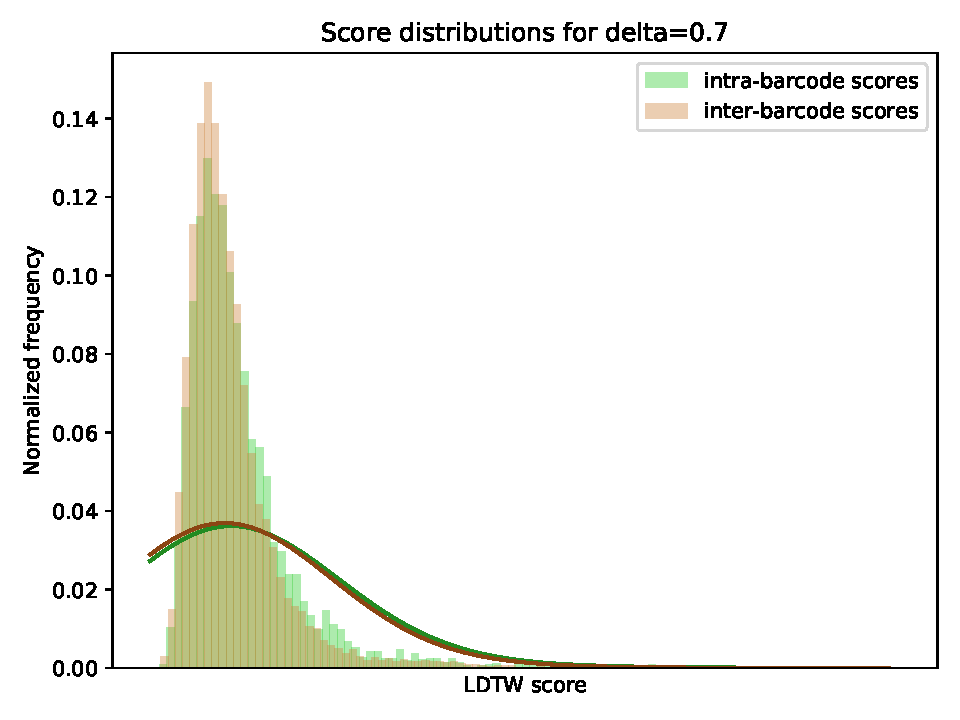
\includegraphics[scale=0.5]{images/delta/delta_raw_70.pdf}

\caption[Score distributions for different values of $\delta$]{This figure displays the changes of LDTW score distributions in terms of different values of $\delta$. For each value of $\delta$ the scores were computed using the same set of squiggles.} \label{fig:deltas_collage}
\end{figure}

Table \ref{tab:delta_measures} shows the values of  $\textbf{BC}$ and $\textbf{OA}$ for different values of $\delta$. By examining these values, we have chosen $\delta = 0.5$ and will use this value for the rest of this work.

\begin{figure}[!ht]
    \centering
    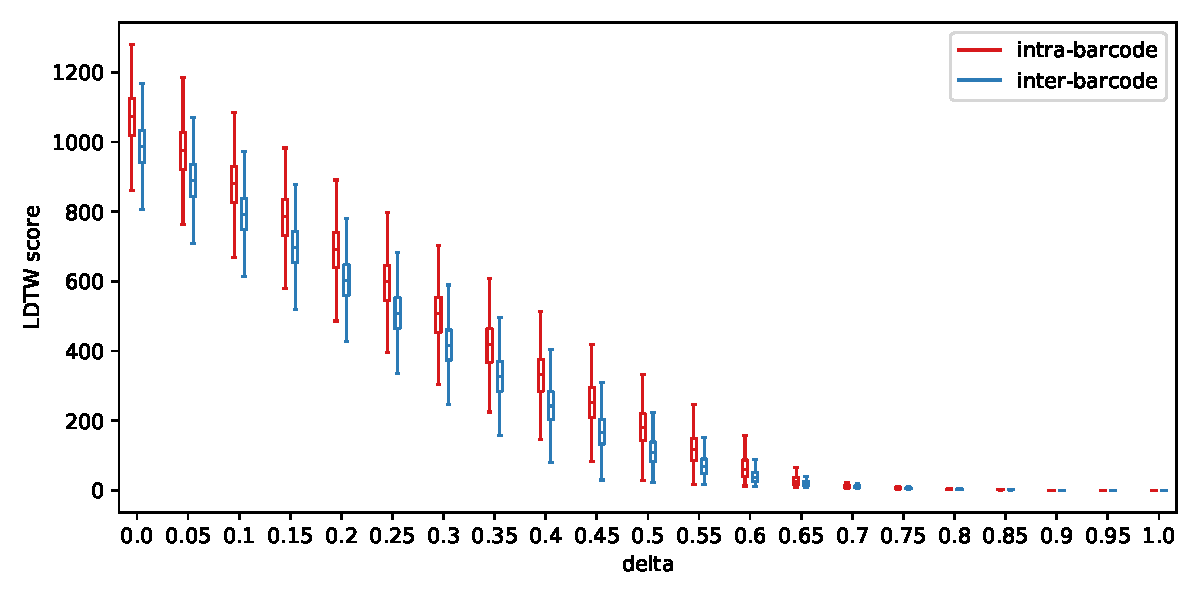
\includegraphics[scale=0.7]{images/delta_raw_boxplot.pdf}
    \caption[Scores dispersion in terms of $\delta$]{This double boxplot graph summarizes how the dispersion of the scores changes in term of $\delta$. As can be seen, the scores around $\delta = 0.5$ result in non-overalapping lower quartile of intra-barcode scores with upper quanrile of inter-barcode scores. Larger values of $\delta$ yield increasingly bigger overlaps.}
    \label{fig:delta_boxplot}
\end{figure}

\begin{figure}[!ht]
    \centering
    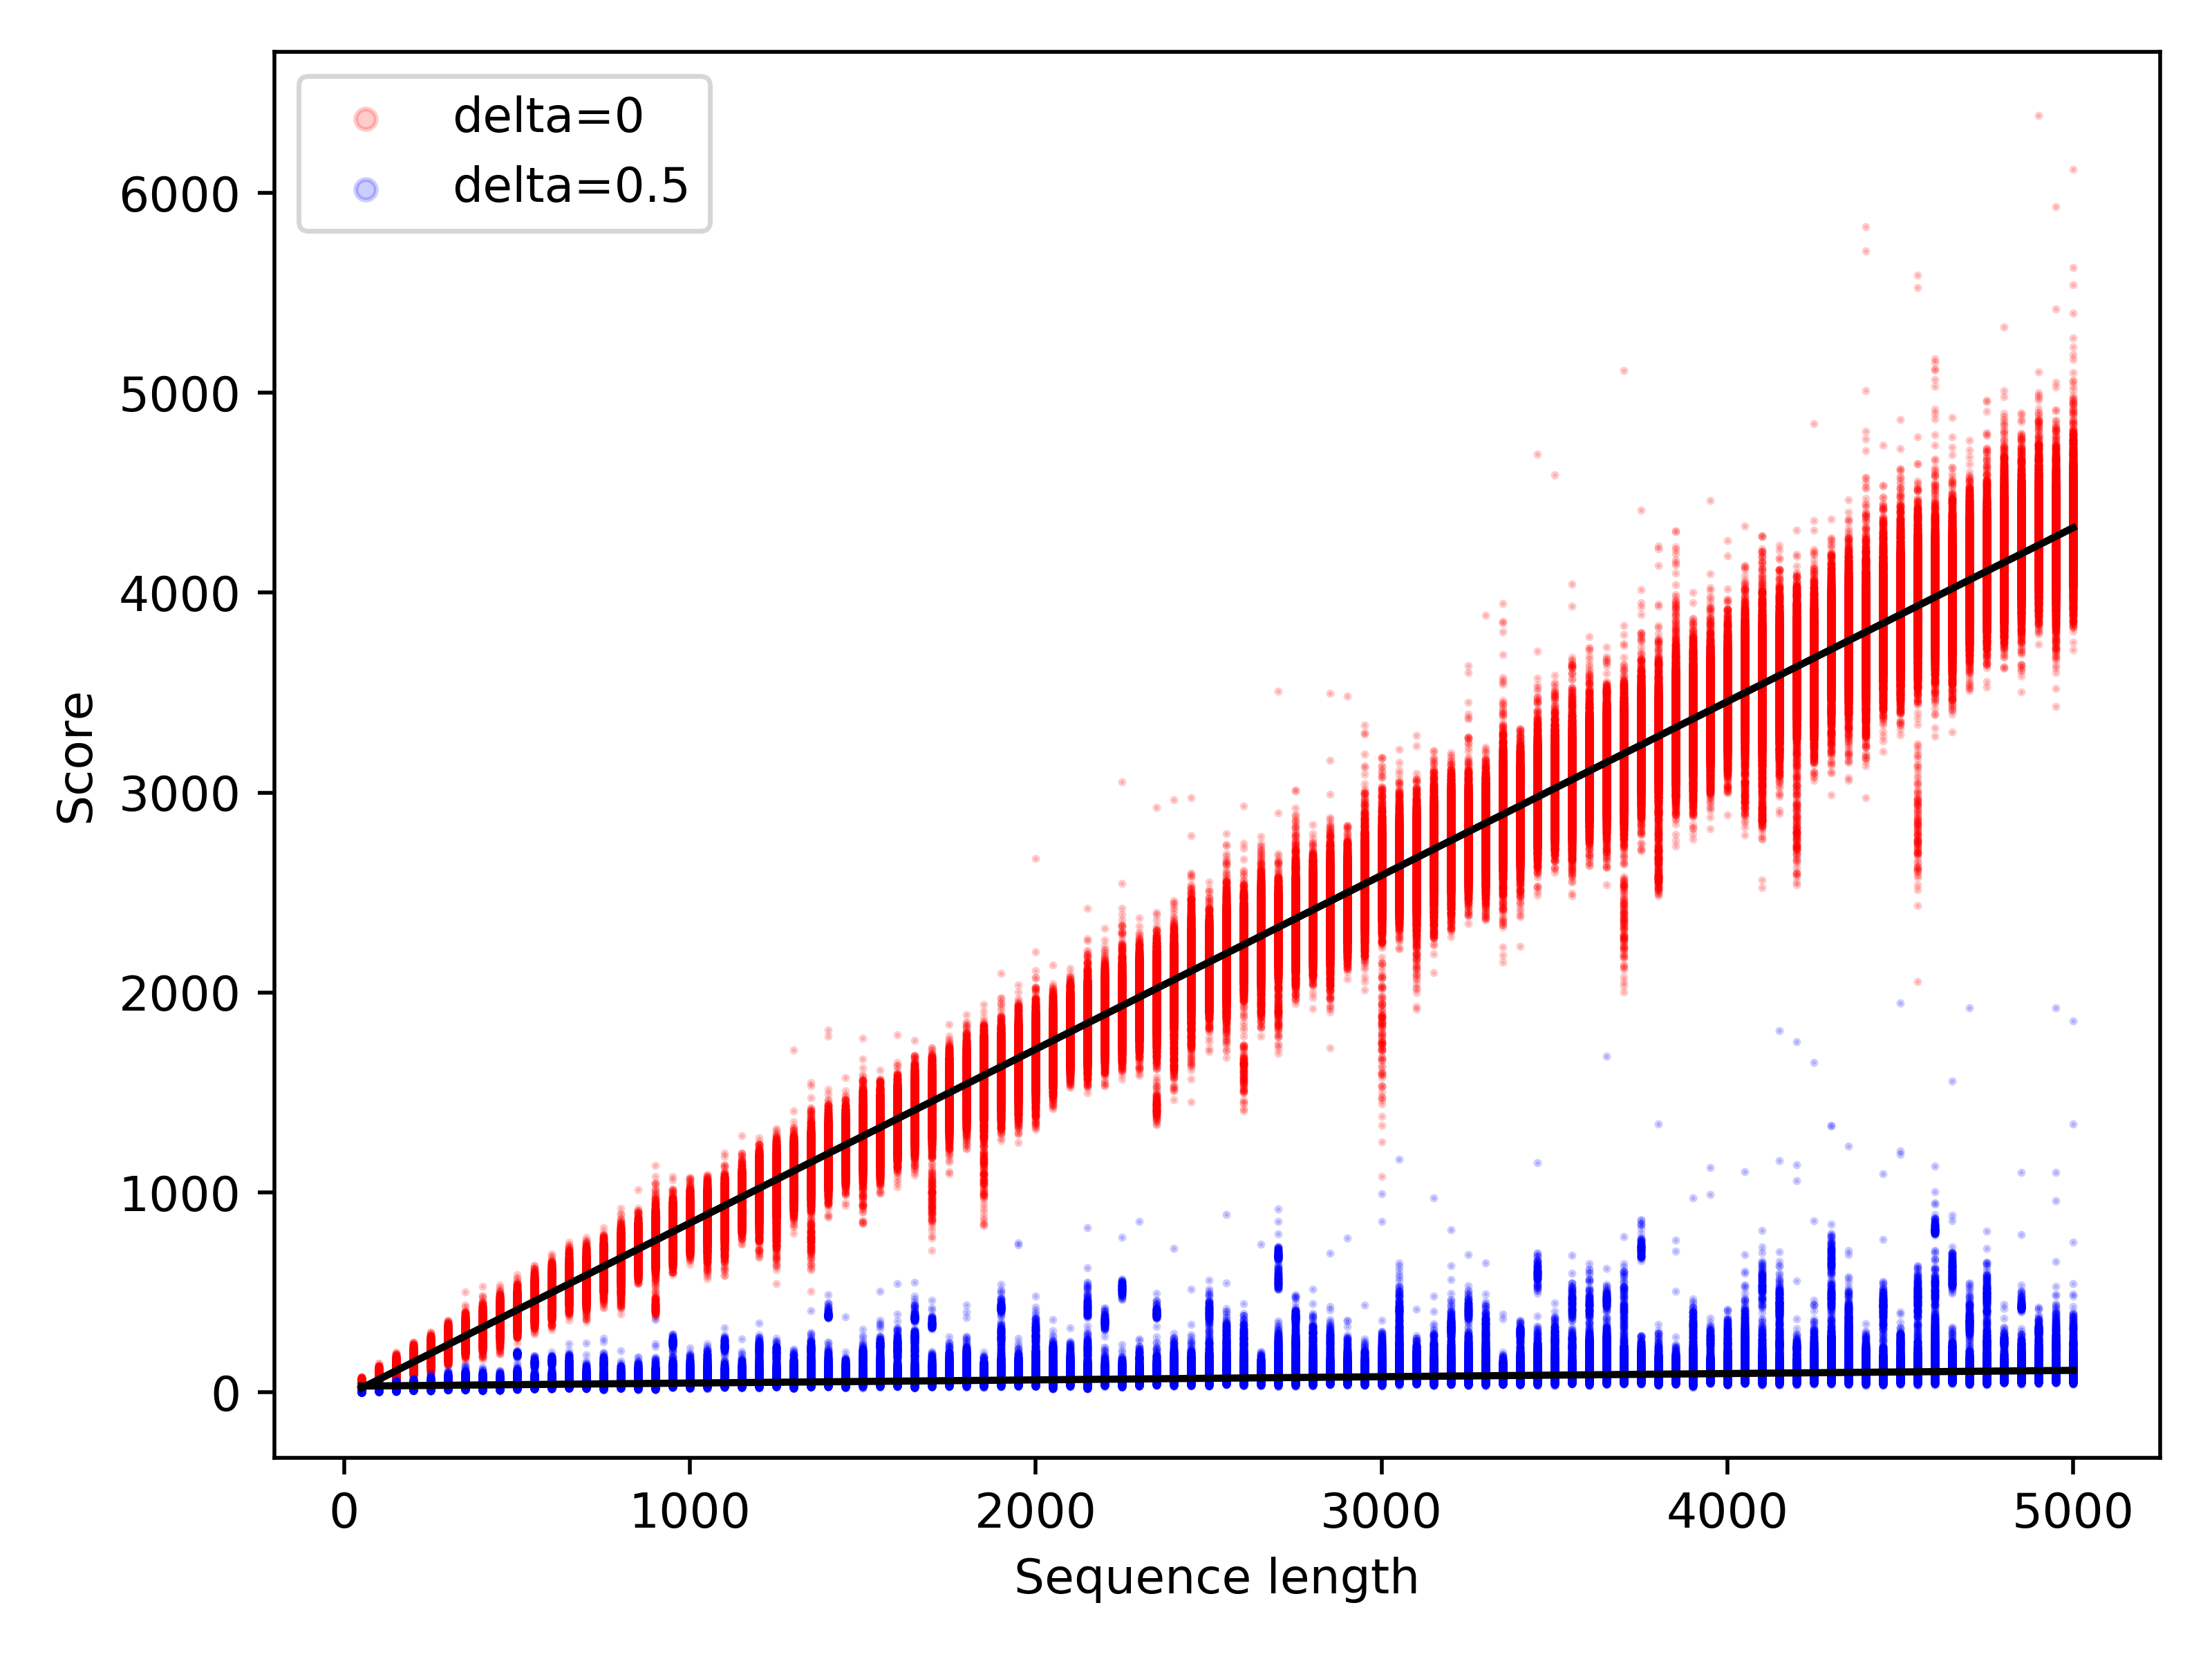
\includegraphics[scale=0.8]{images/rand_align_dpi.png}
    \caption[Random sequences LDTW scores]{The scatter plot depicting the relationship between the length of the random sequences and the similarity score given by LDTW. The black lines are the corresponding estimations of the slope given by the Theil-Sen regression impleneted in \texttt{scikit-learn} library \cite{scikit-learn}.}
    \label{fig:rand_align}
\end{figure}

To see how the $\delta$ correction performs in alignments of random sequences, we performed the following experiment. For each sequence length $\ell = 50, 100, 150, ..., 5000$ we randomly sampled $100$ squiggles of length $\ell$ out of our training data by picking a position in the squiggle uniformly at random and extracting the window of $\ell$ signal values. Subsequently we computed the LDTW scores between all pairs of the $100$ squiggles. This process was performed once for $\delta = 0$ and once for $\delta = 0.5$. The LDTW scores are scattered across the sequences length $\ell$ in Fig. \ref{fig:delta_samples}. We can see that while $\delta = 0$ allows for the scores to grow linearly with length, the $\delta = 0.5$ option shows almost no growth at all.


\section{Assessing the Discriminative Power}
The most desirable property of our LDTW similarity measure is to have discriminative power, i.e. to be able to distinguish the barcode match or mismatch solely on the basis of the alignment score - we will refer to this ability as how well our metric \textit{separates} the space of squiggles. To assess the discriminative power of our metric, we are going to inspect its ability to separate the barcode classes by examining a few cases by hand, as well as visualize the quality of the separation by projecting the LDTW scores to pointwise distances in a Cartesian space.

\begin{figure}[!ht]
    \centering
    \subfloat[$\delta = 0$]
    {{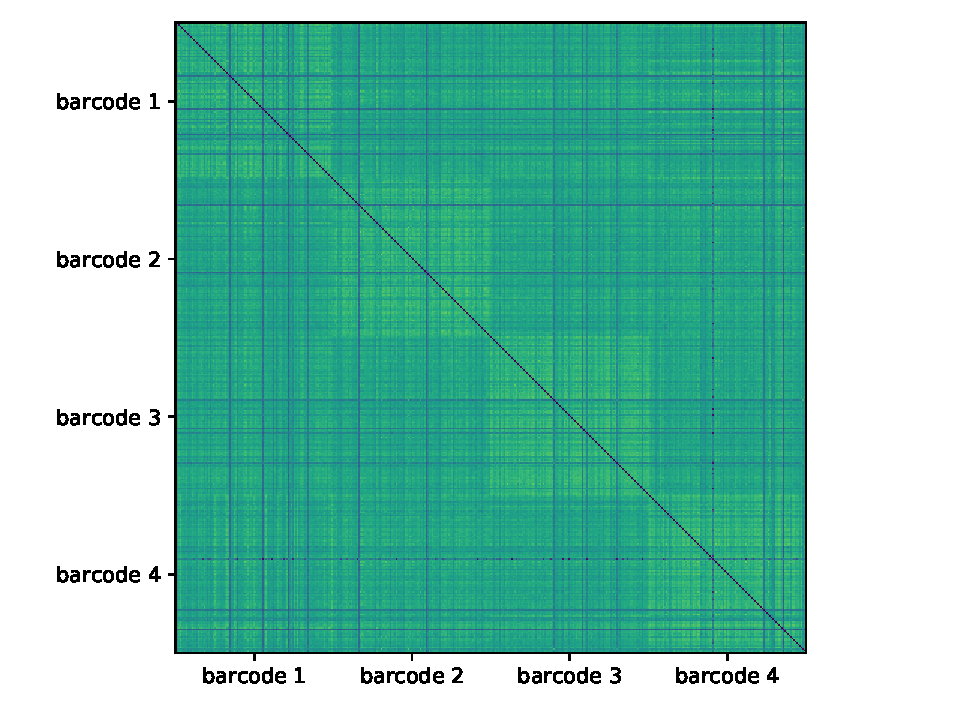
\includegraphics[width=7cm]{images/2000_raw_delta0.pdf} }}%
    \qquad
    \subfloat[$\delta = 0.5$]
    {{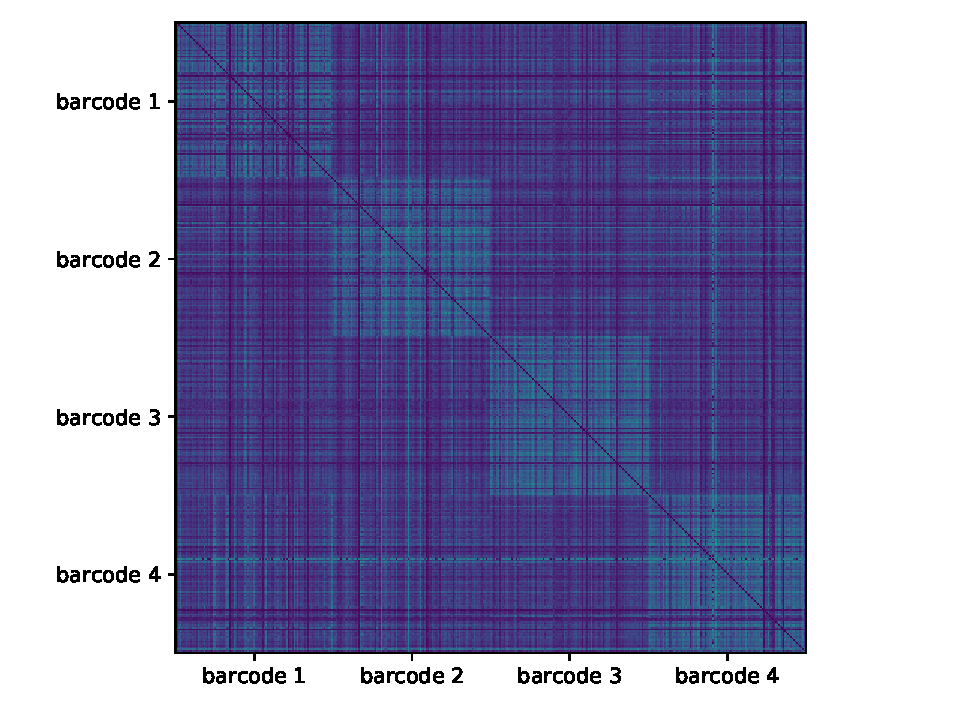
\includegraphics[width=7cm]{images/2000_raw_delta5.pdf} }}%
    \caption[Prefix sample LDTW scores]{Score matrices corresponding to all-pair LDTW similarities of a perfectly balanced sample of $500$ squiggles from each of the barcodes $1-4$. The same score matrix is computed for both choices of $\delta$ in $\{0, 0.5\}$. Only prefix scores were considered.}
    \label{fig:delta_samples}
\end{figure}

\subsection{Examination by Hand}
We looked at several tens of alignments between each pair of barcode classes in effort to observe the behavior of our LDTW similarity measure on concrete examples. One of the things that we noticed was that the final alignment score is occasionally rather relative. By 'relative' we mean that we sometimes cannot differentiate between a barcode match or mismatch solely on the basis of the alignment score. We attribute this phenomenon to the nature of our scoring scheme, which is in fact a non-increasing function of the distances between squiggle points. Therefore it is possible to happen that shorter subsequences of very similar shapes in mismatched squiggles can actually yield higher scores than barcode matches in lesser quality squiggles. An example of four LDTW alignments can be seen in Fig. \ref{fig:LDTW_alignments}), where we can observe full-length barcode alignments of pairs from the same barcode class, but only short alignments (probably corresponding to flank sequences discussed in Sec. \ref{sec:data_structure}) in pairs from different classes. Overall, from examining random pairs of both intra-class and inter-class alignments, we can conclude that the LDTW similarity with $\delta = 0.5$ works satisfactorily and the clusters are well pronounced (see Fig. \ref{fig:delta_samples}). To gain a more enlightening view, however, we need more power tools.

\begin{figure}[ht] % "[t!]" placement specifier just for this example
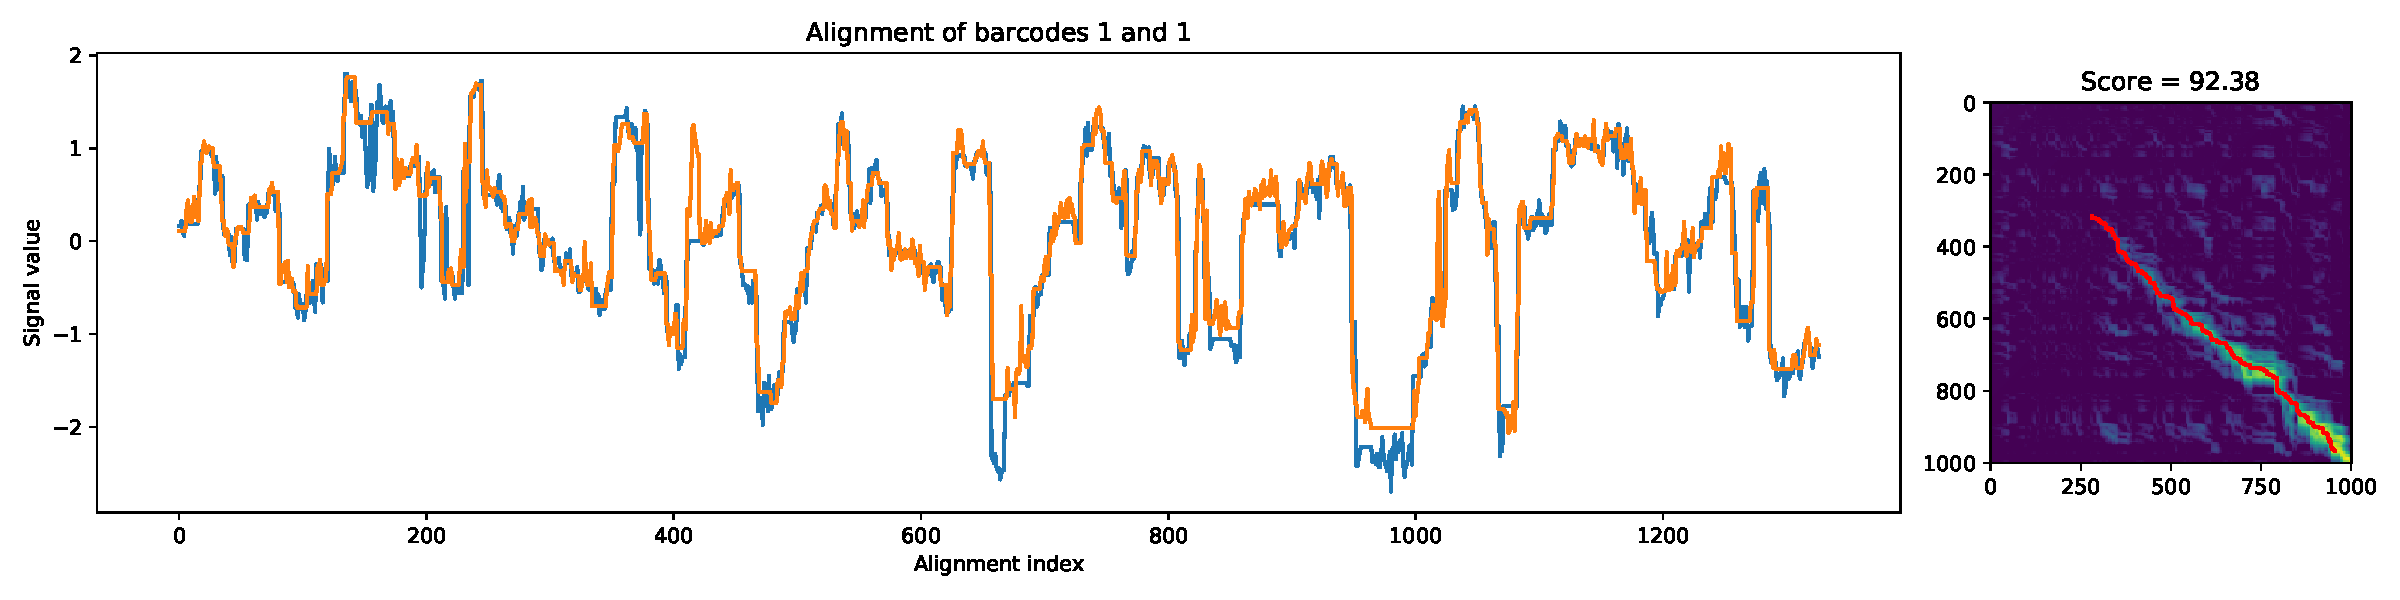
\includegraphics[scale=0.4]{images/bc1_bc1_1823_1739.pdf}
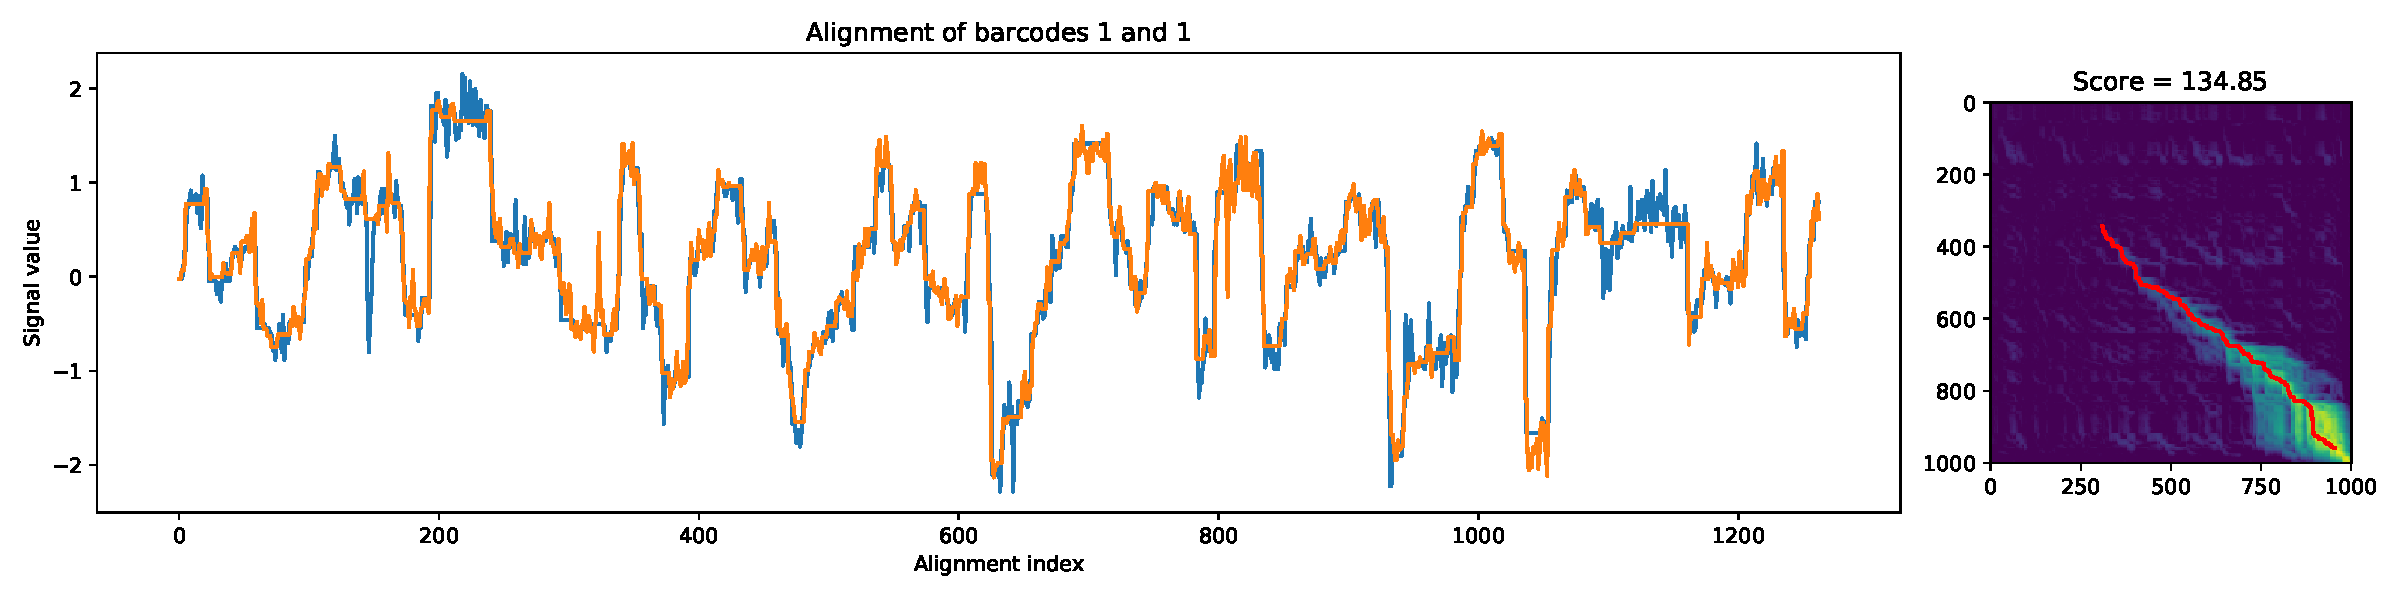
\includegraphics[scale=0.4]{images/bc1_bc1_1902_1453.pdf}

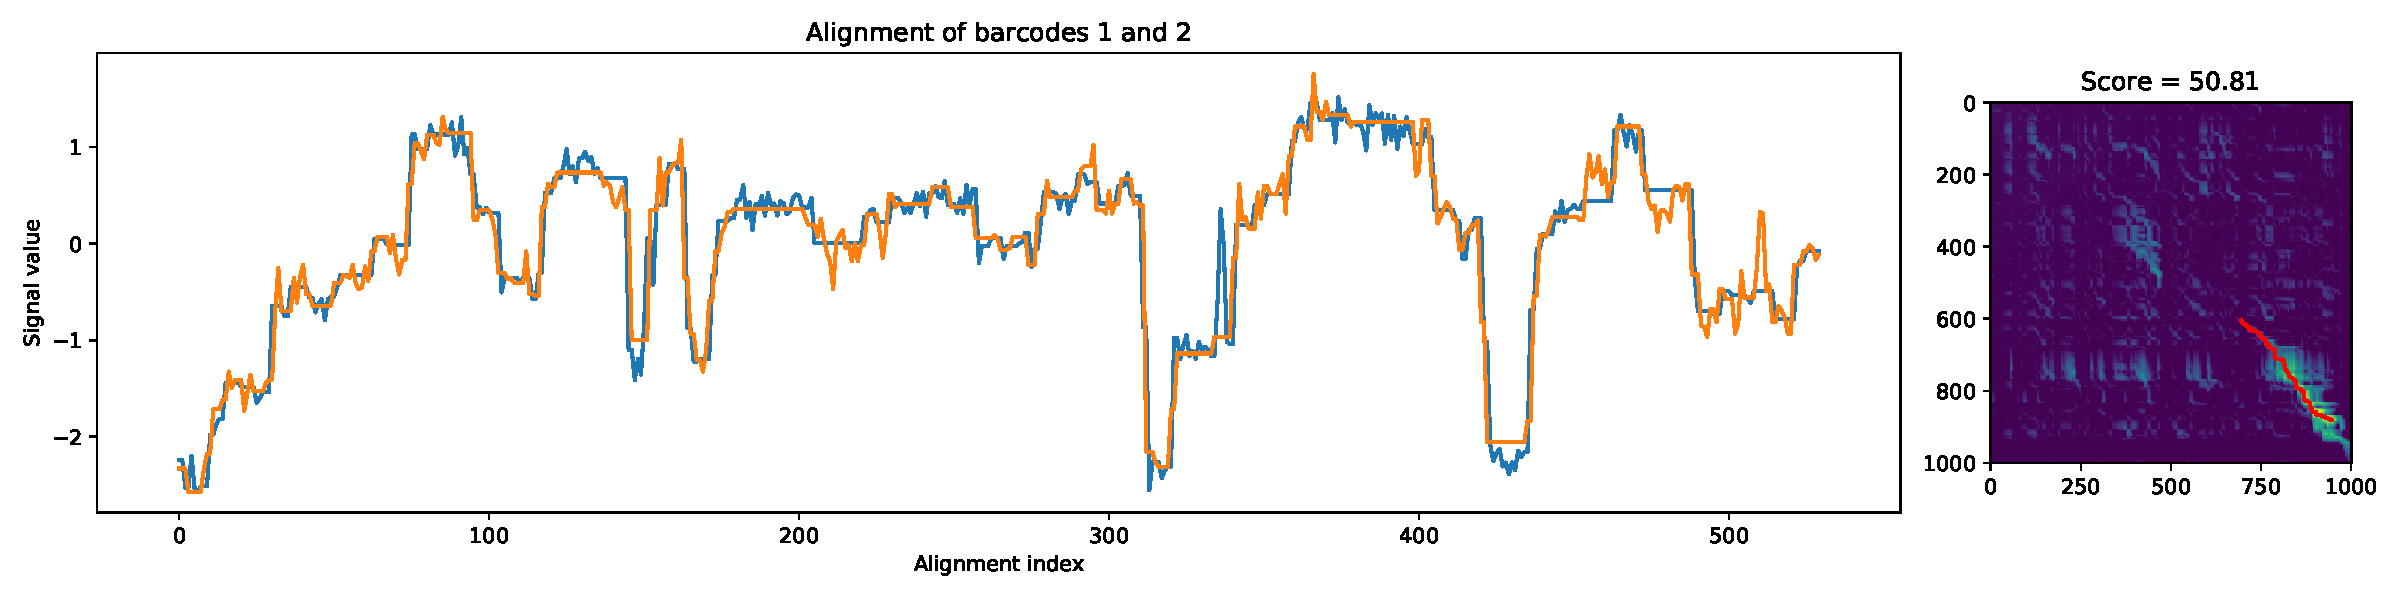
\includegraphics[scale=0.4]{images/bc1_bc2_1698_2660.pdf}
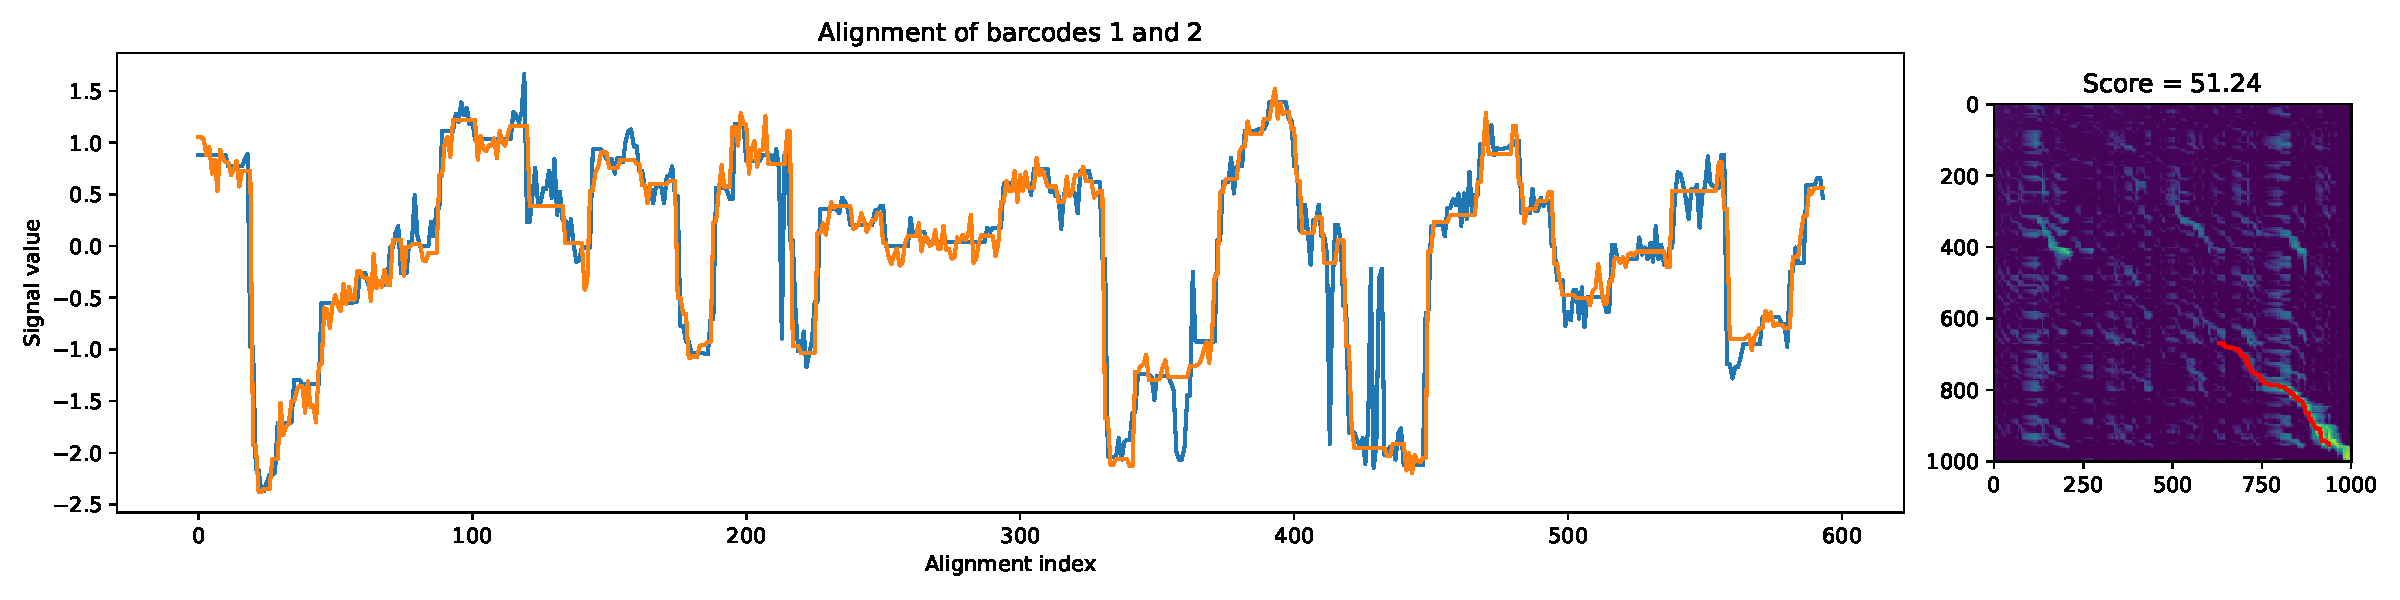
\includegraphics[scale=0.4]{images/bc1_bc2_2172_2742.pdf}

\caption[LDTW alignments between two pairs of squiggles]{LDTW alignments between two pairs of squiggles with barcode $1$ and another two alignments between pairs of squiggles with barcodes $1$ and $2$.} \label{fig:LDTW_alignments}
\end{figure}

\subsection{Multidimensional Scaling}
One of the methods that enable us to visualize some notion of a metric defined on pairs of objects and uncover the hidden structure of the measured data is \textit{Multidimensional Scaling} (MDS) \cite{kruskal1978multidimensional}. MDS usually refers to a whole family of methods used to perform this task in different settings \cite{mead1992review}. MDS takes as an input a distance/similarity matrix $D_{n\times n}$ (an entry $d_{ij}$ represents the distance/similarity of $i$-th and $j$-th object) of $N$ objects in total and an integer $M$ determining the embedding dimension. Its output is a set of corresponding $N$ points in $M-$dimensional Euclidean space such that the pairwise Euclidean distances between the points reflect the relative metric values in the matrix $D$ \cite{kruskal1978multidimensional, mead1992review}.

Most MDS methods assume that (in case of a similarity) the input similarity measure $s(\cdot, \cdot)$ fulfills some basic properties of a metric, most commonly it is (\cite{mead1992review}) :

\begin{enumerate}
    \item (Non-negativity) $s_{ij} \geq 0$
    \item (Identity of indiscernibles) $s_{ij} = 0$ if and only if $i = j$
    \item (Symmetricity) $s_{ij} = s_{ji}$
\end{enumerate}

These $3$ conditions are fulfilled for our LDTW similarity function $s(\cdot, \cdot)$: non-negativity and identity are obvious from the construction. Symmetricity is the corollary of the symmetricity of classical DTW and the symmetricity of our scoring function.

MDS in general tries to minimize a function called \textsc{stress}, which measures the sum of residuals the embedding. Let $D$ be the input matrix of observed measurements and $\vec{x}_1, ..., \vec{x}_n \in \mathbb{R}^m$ be the vectors of coordinates in the $m$-dimensional embedding. Let $\widehat{D}_{n \times n}$ be a matrix where $\widehat{d}_{i,j} = ||x_i - x_j||$ and $||.||$ is the Frobienus norm \cite{frobnorm}. The \textsc{stress} is then defined as (\cite{kruskal1964nonmetric}):

\begin{equation}
    \textsc{stress}_{D}(x_1, ..., x_n) = \frac{
        %\sqrt{ \sum_{i=1}^n \sum_{j=1}^n \Big( d_{ij} - ||\vec{x}_i - \vec{x}_j|| \Big)^2 }
        ||D-\widehat{D}||
    }{
        %\sqrt{ \sum_{i=1}^n \sum_{j=1}^n d_{ij}^2 }
        ||D||
    } =
    \frac{
        \sqrt{ \sum_{i=1}^n \sum_{j=1}^n \Big( d_{ij} - \sqrt { \sum_{k=1}^m \big(
            \vec{x}_i - \vec{x}_j \big)^2 }
        \Big)^2 }
    }{
        \sqrt{ \sum_{i=1}^n \sum_{j=1}^n d_{ij}^2 }
    }
    \label{eq:stress}
\end{equation}

The denominator is present only for the purpose of rescaling the stress value to a range $[0, 1]$ and therefore irrelevant to the optimisation. \textsc{stress} minimization is a complicated optimization problem, often solved by the SMACOF (Scaling by MAjorizing a COmplicated Function) algorithm \cite{smacof}. \textsc{stress} is simultaneously a way of measuring the 'goodness of fit' \cite{kruskal1964nonmetric}, so we will report with along with the actual projection.

\begin{figure}[!ht]
    \centering
    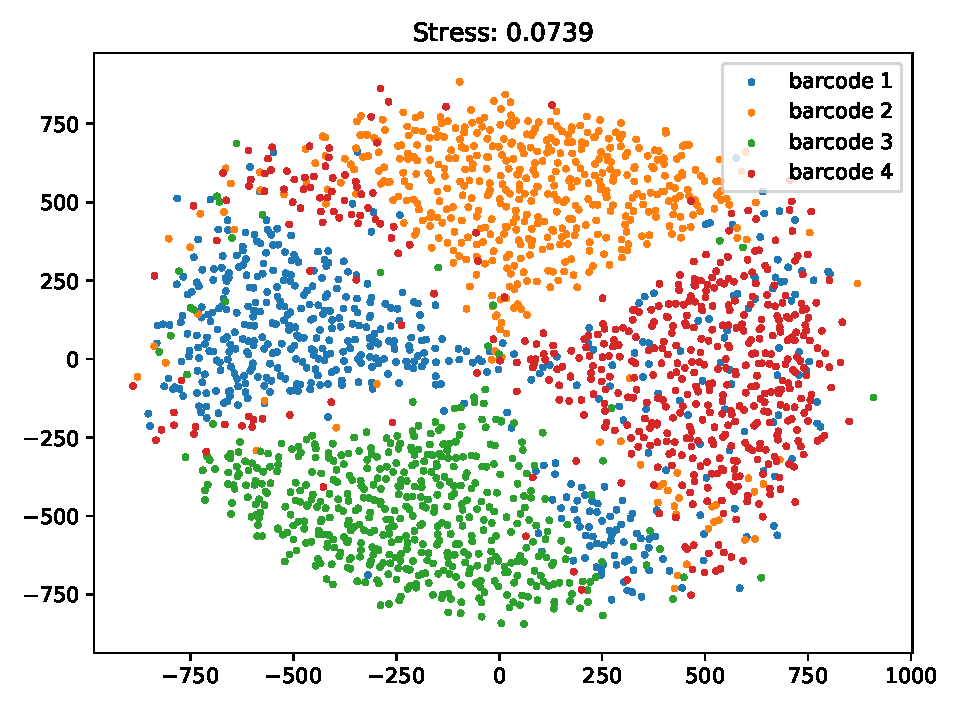
\includegraphics[width=15.5cm]{images/mds2000_2D.pdf}
    \caption[MDS projection to $2$D space]{MDS projection of $2000$ reads to $2$D Cartesian space. We can see that the barcode pairs $(1, 3)$ and $(2, 4)$ are of higher similarity than other pairs, resulting in non-trivial misplacement of some orange reads. Otherwise, the reads seem to be split relatively well.}
    \label{fig:2000_MDS_2D}
\end{figure}

\begin{figure}%
    \centering
    \subfloat[]
    {{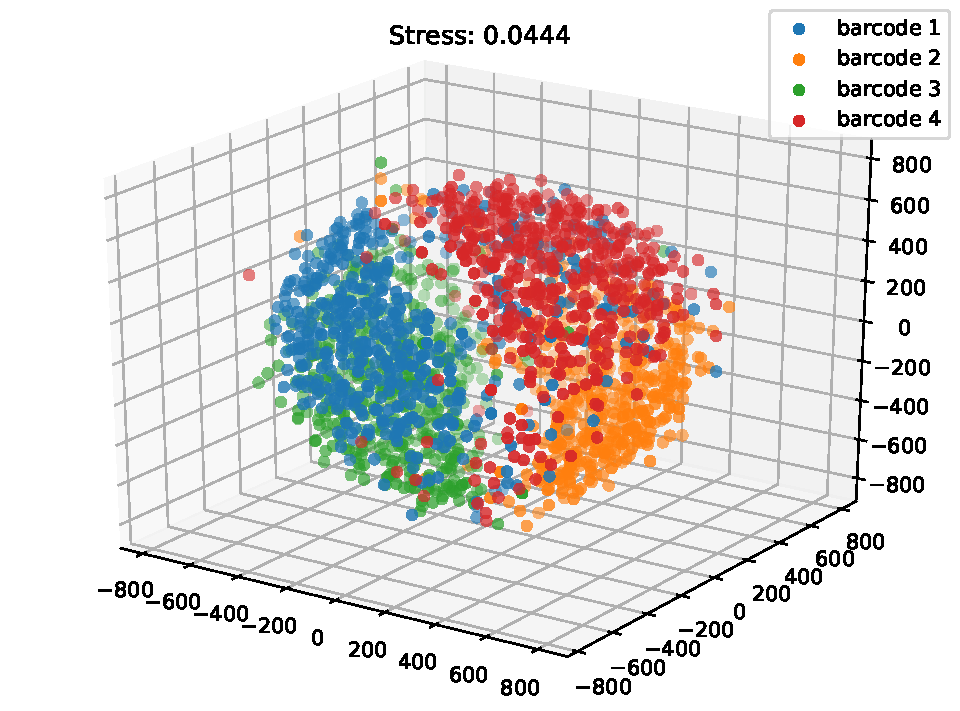
\includegraphics[width=14cm]{images/mds2000_3D_1.pdf} }}%
    \qquad
    \subfloat[]
    {{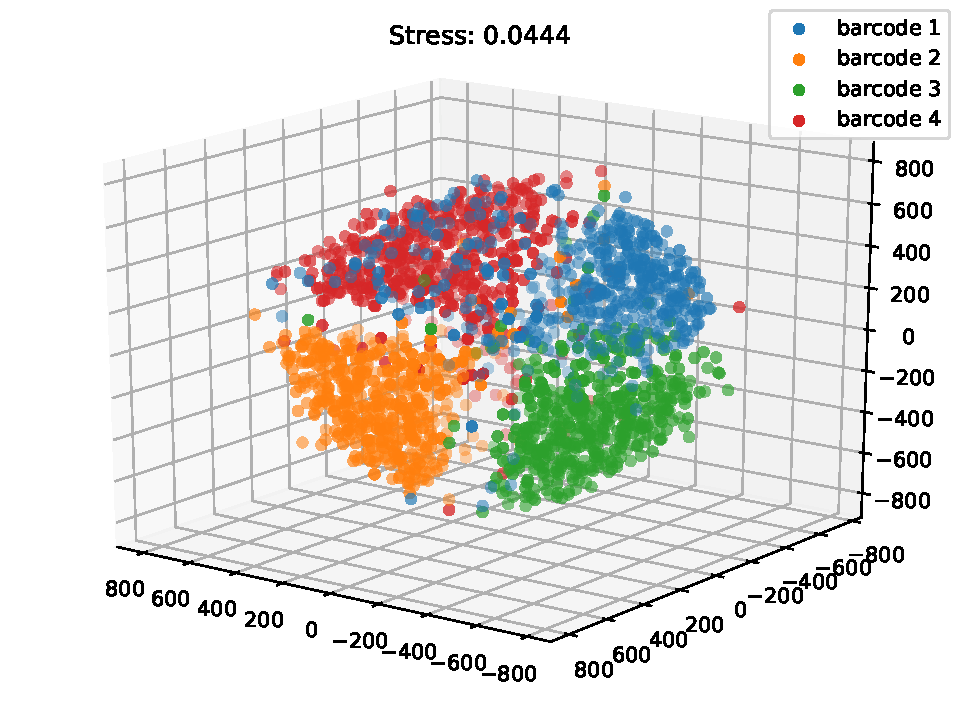
\includegraphics[width=14cm]{images/mds2000_3D_3.pdf} }}%
    \caption[MDS projection to $3$D space]{MDS embedding into a $3$D Cartesian space in two different views. As we can see, the extra dimension allowed for a better layout of the data points and the \textsc{stress} level is at half in comparison with the $2$D embedding in Fig \ref{fig:2000_MDS_2D}.}
    \label{fig:2000_MDS_3D}
\end{figure}

From the Fig. \ref{fig:2000_MDS_2D} and \ref{fig:2000_MDS_3D} we can conclude that the classes are reasonably well separated by the LDTW score, with relatively small overlap. An interesting phenomenon that appears to be present is that some point belonging to the barcode $1$ are mixed well into the cluster of barcode $4$, but not the other way around.

\subsection{Triangle Inequality}
Proving that the triangle inequality holds for our LDTW metric would mean that LDTW on the set of squiggles is in fact a metric space. The triangle inequality itself would give us the possibility to leave out redundant computations in the clustering phase, such as in accelerated $k$-means by Elkan et al. \cite{elkan2003using}. This would provide to be especially useful as our LDTW is rather expensive in terms of computation time.

However, it is known that the classic DTW algorithm as metric does not satisfy the triangle inequality \cite{yi1998efficient}. Not surprisingly the same is true for our LDTW algorithm, which we proved empirically by observing the scores of all pairs in sample of squiggles. However, we found that

\begin{equation}
    P \Big[ \text{LDTW}(p_i, p_j) \leq \text{LDTW}(p_i, p_k) + \text{LDTW}(p_k, p_j) \Big] \approx 0.91,
\end{equation}

where $p_i, p_j, p_k$ are \textbf{p}refixes from randomly sampled squiggles. In other words, the triangle inequality holds in $\approx 91\%$ of all possible cases, which renders it possible to use from a probabilistic point of view, where we could work with a certain probability of a tree reads satisfying the inequality. Moreover it tells us that our metric behaves meaningfully in most cases.

Furthermore, we found that

\begin{multline}
    P \Big[ \big( \text{LDTW}(p_i, p_j) + \text{LDTW}(s_i, s_j) \big) \leq \big( \text{LDTW}(p_i, p_k) + \text{LDTW}(s_i, s_k) \big) + \\ + \big( \text{LDTW}(p_k, p_j) + \text{LDTW}(s_k, s_j) \big) \Big] \approx 0.95,
\end{multline}

where $s_i, s_j, s_k$ are the corresponding squiggle suffixes. In other words, summing together the LDTW scores form prefixes and suffixes increases the resemblance of a metric space.

\subsection{Summary}
We have designed a similarity measure that can be used co compare squiggles on the barcode equality.
Our measure should be invariant to the particular barcodes that are being used in the experiment.